% !TEX TS-program = pdflatex
% !TEX encoding = UTF-8 Unicode

% This is a simple template for a LaTeX document using the "article" class.
% See "book", "report", "letter" for other types of document.

\documentclass[11pt]{article} % use larger type; default would be 10pt

\usepackage[utf8]{inputenc} % set input encoding (not needed with XeLaTeX)

%%% Examples of Article customizations
% These packages are optional, depending whether you want the features they provide.
% See the LaTeX Companion or other references for full information.

%%% PAGE DIMENSIONS
\usepackage{geometry} % to change the page dimensions
\geometry{a4paper} % or letterpaper (US) or a5paper or....
\geometry{margin=2in} % for example, change the margins to 2 inches all round
% \geometry{landscape} % set up the page for landscape
%   read geometry.pdf for detailed page layout information

\usepackage{graphicx} % support the \includegraphics command and options
\usepackage{fullpage}

% \usepackage[parfill]{parskip} % Activate to begin paragraphs with an empty line rather than an indent

%%% PACKAGES
\usepackage{booktabs} % for much better looking tables
\usepackage{array} % for better arrays (eg matrices) in maths
\usepackage{paralist} % very flexible & customisable lists (eg. enumerate/itemize, etc.)
\usepackage{verbatim} % adds environment for commenting out blocks of text & for better verbatim
\usepackage{subfig} % make it possible to include more than one captioned figure/table in a single float
% These packages are all incorporated in the memoir class to one degree or another...

%%% HEADERS & FOOTERS
\usepackage{fancyhdr} % This should be set AFTER setting up the page geometry
\pagestyle{fancy} % options: empty , plain , fancy
\renewcommand{\headrulewidth}{0.5pt} % customise the layout...
\lhead{}\chead{Smart Refrigerator Proposal}\rhead{}
\lfoot{}\cfoot{\thepage}\rfoot{}
\addtolength{\topskip}{+0.5cm}

%%% SECTION TITLE APPEARANCE
\usepackage{sectsty}
%\allsectionsfont{\sffamily\mdseries\upshape} % (See the fntguide.pdf for font help)
% (This matches ConTeXt defaults)

%%% ToC (table of contents) APPEARANCE
\usepackage[nottoc,notlof,notlot]{tocbibind} % Put the bibliography in the ToC
\usepackage[titles,subfigure]{tocloft} % Alter the style of the Table of Contents
%\renewcommand{\cftsecfont}{\rmfamily\mdseries\upshape}
%\renewcommand{\cftsecpagefont}{\rmfamily\mdseries\upshape} % No bold!

\usepackage{amsmath}
%\usepackage{amsfonts}
%\usepackage{amssymb}
\usepackage[normalem]{ulem}
\usepackage{url}
\usepackage{graphicx}

%1 Exercise number
%2 Exercise name
%3 Date performed
%4 Date submitted
\newcommand{\coversheet}[4]{
  \begin{titlepage}
    \setlength\topmargin{2in}
    \begin{center}
      \Huge\textsc{Smart Refrigerator Proposal}\\
      \vspace{.125in}
      \hrule
      \vspace{.125in}
      \normalsize
      \today \\
      \vspace{.375in}
      This project will develop a prototype “Smart Refrigerator” system, which will monitor grocery items purchased by the user in order to reduce food waste and facilitate efficient shopping habits. 

    \end{center}
    \vfill
    \hspace{4.2in} Steven Strapp - ses6498@rit.edu
    
    \noindent \hspace{4.2in} Computer Engineering Year 4

    \noindent \hspace{4.2in} 

    \noindent \hspace{4.2in} Ben Reeves - bpr5171@rit.edu
    
    \noindent \hspace{4.2in} Computer Engineering Year 5

    \noindent \hspace{4.2in} 

    \noindent \hspace{4.2in} Dustin Stroup - dxs2857@rit.edu

    \noindent \hspace{4.2in} Computer Engineering Year 5

    \quad \newline \newline \newline \newline \newline \newline \newline \newline
  \end{titlepage}
}

%1 label
%2 number of variables
%3 kmap label
%4 variables
%5 truth table
%6 Marks
%7 Prime implicants table
%8 Final EQ
\newcommand{\kmap}[8]{
  \begin{center}
    \begin{tabular}{l}
      \multicolumn{2}{c}{\underline{#1}} \\  
        \karnaughmap{#2}{#3}{#4}{#5}{
		#6        
        }
      #8
    \end{tabular}
  \end{center}
  }

%1 figure position
%2 figure scale
%3 path to photo
%4 Caption
%5 reference lable
\newcommand{\pic}[5]{
\begin{figure}[#1]
  \begin{center}
    \includegraphics[scale=#2]{#3}
    \caption{#4}
    \label{#5}
  \end{center}
\end{figure}
}



\begin{document}
\coversheet{V}{\textsc{Kinetis K60 Based Electrocardiogram}}{October 28, 2011}{November 11, 2011}
\setcounter{page}{2}

\addtolength{\topskip}{+0.5cm}
\tableofcontents
\addtolength{\topskip}{-0.5cm}
\pagebreak
\section{Overview}
\subsection{Needs Statement}
The New York Times reports that an average American family of four will account for over 120 pounds of food waste per month and that 27\% percent of all food available will be lost to waste \cite{times}. In addition, other resources are lost due to inefficient shopping practices; forgetting common items or special trips made for recipe ingredients waste time and fuel. A system is required for shoppers both to ensure their purchases are used before expiration and to assist in planning of grocery shopping trips.
\subsection{Objective Statement}
The objective of this project is to design a prototype that will allow a user to track food items in order to reduce waste and improve shopping efficiency. The system will remind the user about items nearing their expiration date and track the frequency of purchased items. From this frequency calculation the system will suggest typical shopping lists. A mobile phone application will provide an interface to the unit to view or create shopping lists and to query inventory.
\subsection{Description}
A UPC scanner will be used to identify items added or removed from the refrigerator's inventory, and a database of UPC codes will translate from the scanned code to an item description. Two inventory databases will be maintained: one linking UPC codes to product descriptions and another to store items currently checked into the refrigerator and thier expiration dates. A central processing platform on the base station will be used to decode UPC information and to interact with the databases. This processing platform will provide a web interface accessible via a web browser or an Android mobile device. A display on the main unit will allow users to review the current inventory, with expiration dates, and will provide additional information when adding or removing items. The base station, web and mobile interfaces can also be used to display the current inventory and suggested shopping lists. The mobile application will interact with the same web interface but will provide a graphical interface optimized for smaller displays. The system will continually estimate the purchasing frequency for items and will use this information, combined with the expiration and purchase dates, to suggest shopping lists. In addition to shelf life, temperature is also a critical factor for food storage systems. To address this need, the system will incorporate a temperature sensor and the temperature information will be accessible through the base station application.
\newline \quad \newline
A high level system diagram which partitions major components is shown in Figure \ref{fig:sysdiag}.
\begin{figure}[h]
\begin{center}
\vspace{0.5cm}
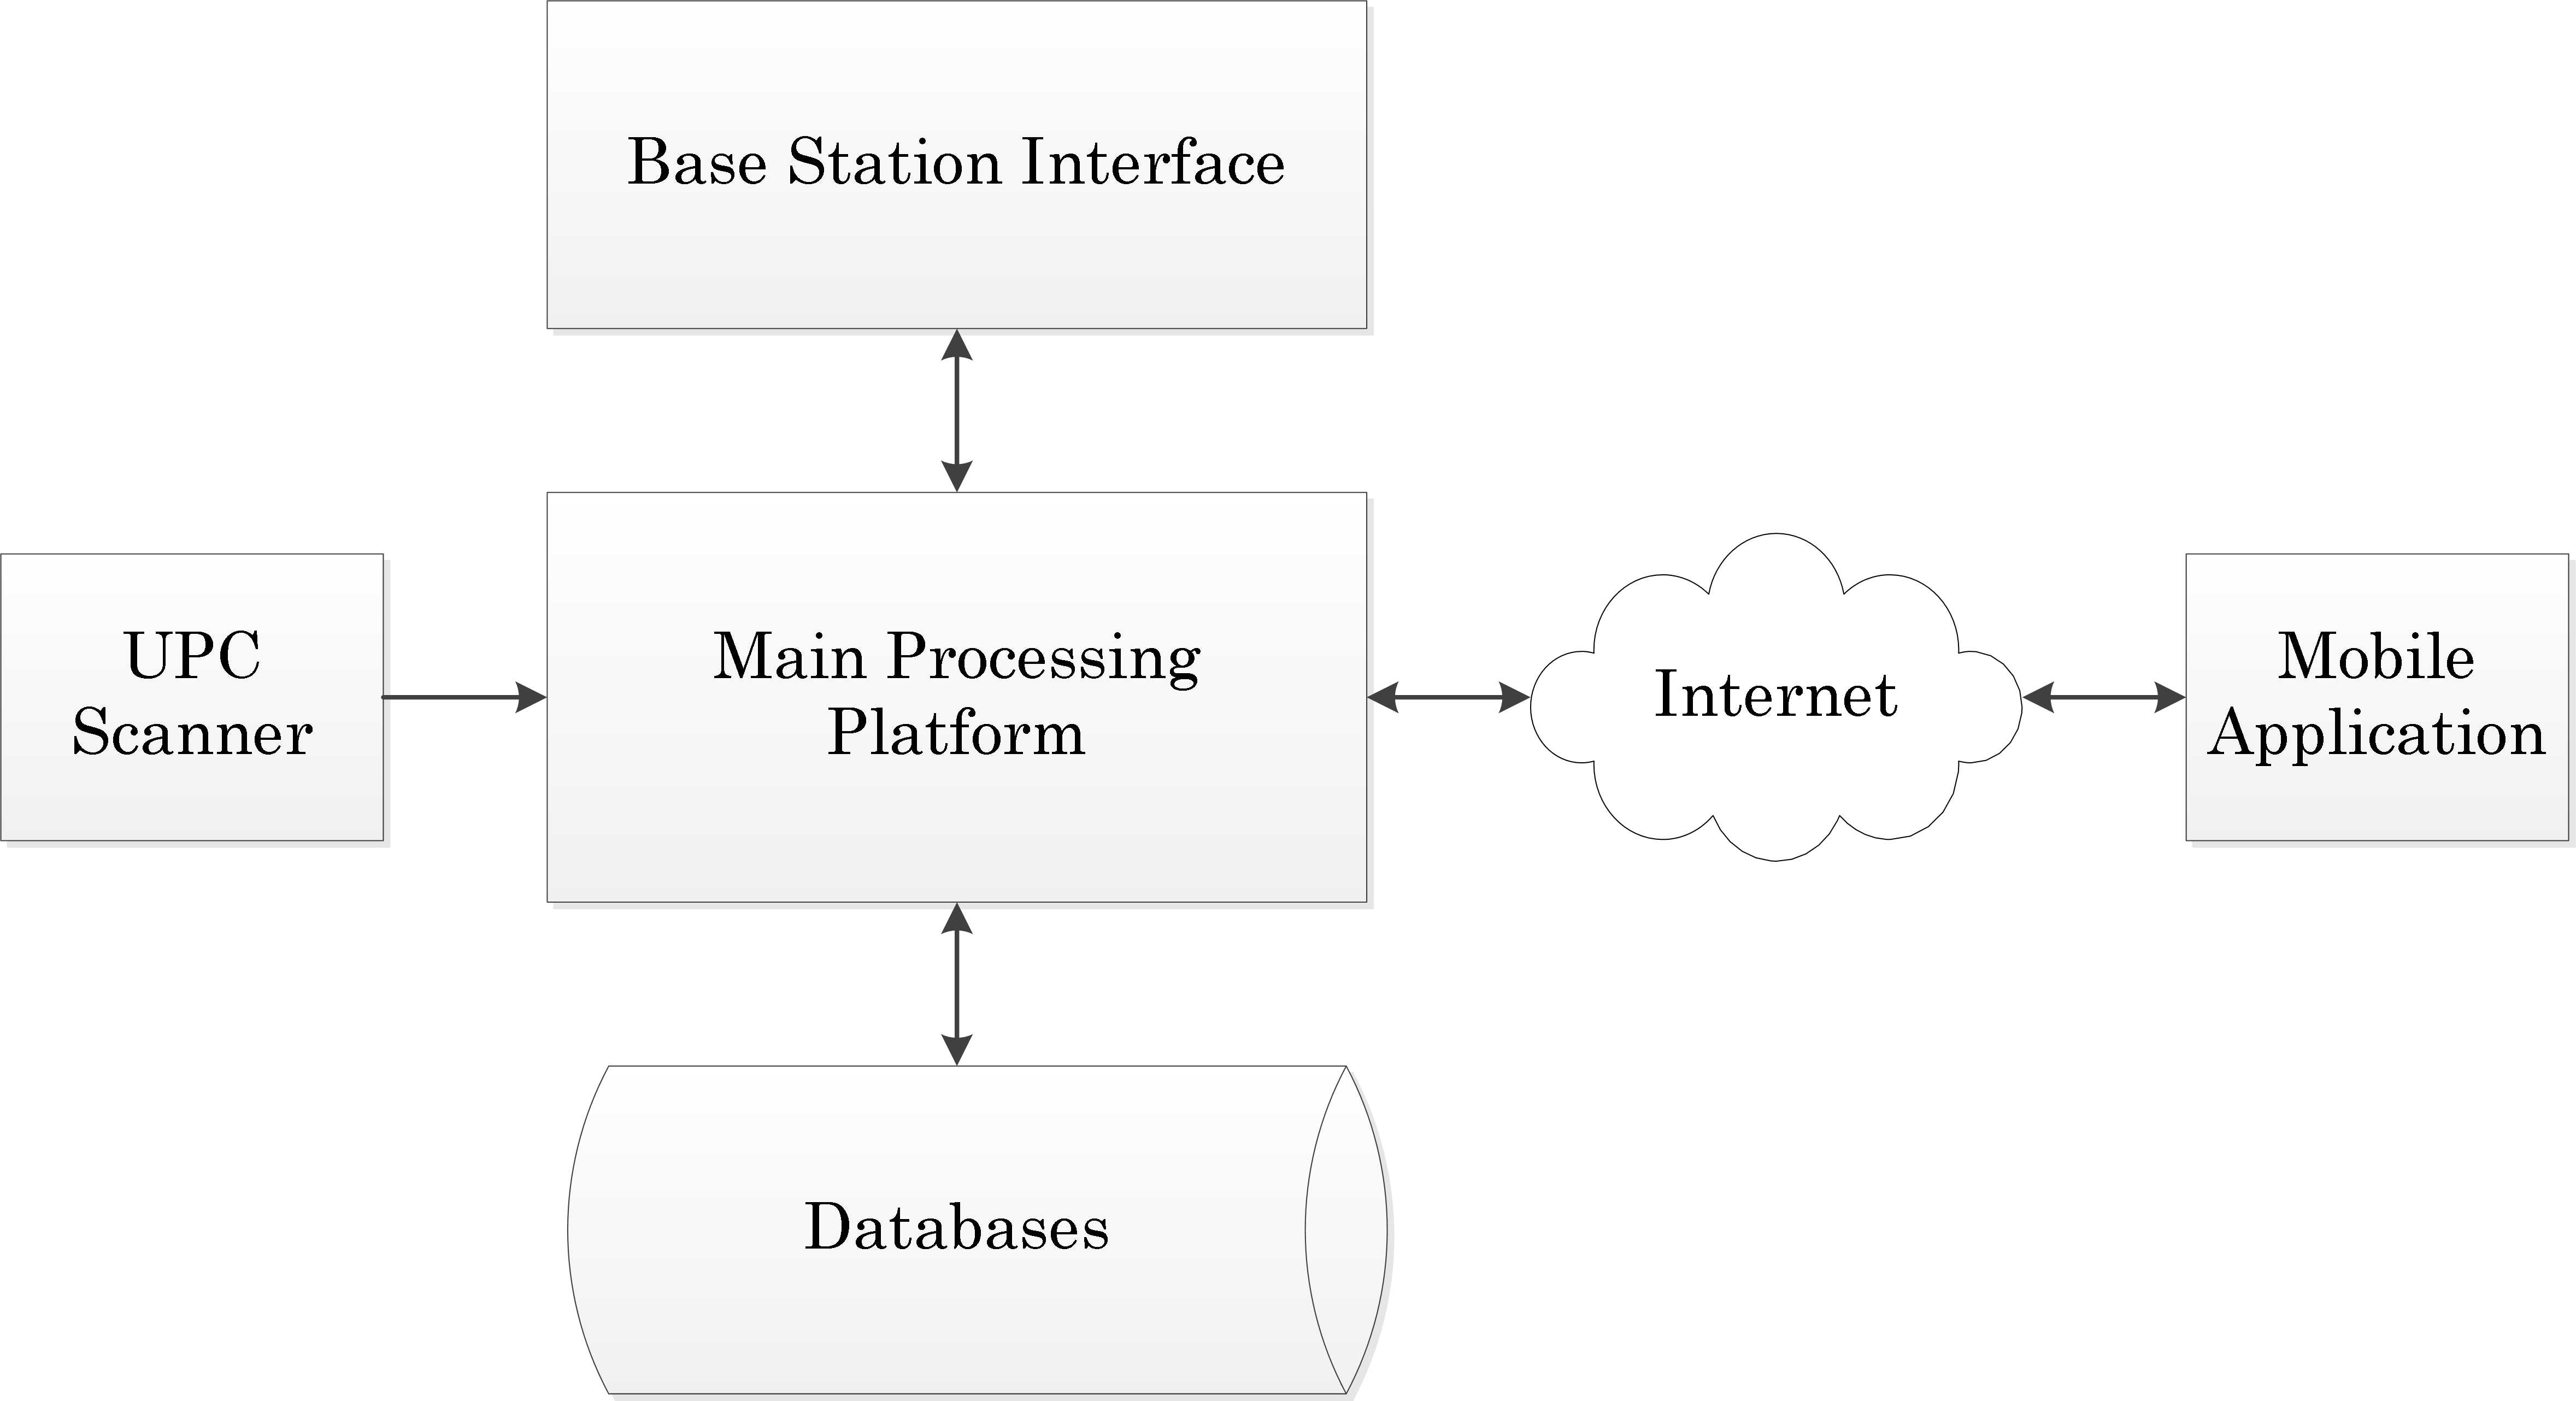
\includegraphics[scale=0.5]{../graphics/HighestLevelDiagram}
\caption{High Level System Diagram}
\label{fig:sysdiag}
\end{center}
\end{figure}
\pagebreak
\section{Requirements Specification}
\subsection{Customer Needs}
\begin{enumerate}
\item The system should provide an intuitive and easy to use graphical interface.
\item The system should require minimal user input.
\item The system should be able to scan product codes and identify corresponding items quickly.
\item The system should provide secure remote access.
\item The system should report items nearing expiration.
\item The system should provide access to the current inventory.
\item The system should provide a method to create and edit shopping lists.
\item The system should recommend shopping lists which accurately reflect buying habits.
\item The system should function as an add-on to an existing refrigerator or pantry.
\item The system should indicate if food products are stored at an unsafe temperature.
\end{enumerate}
\pagebreak
\subsection{Engineering Specifications}
\begin{table}[h!]
\begin{center}
\begin{tabular}{| p{1.2in} | p{2.5in} |p{2.5in} |}
\hline
Customer Need & Engineering Requirement & Justification \\
\hline
2,3 &A. An off-the-shelf UPC scanner should be used to input items. & A UPC scanner can read product codes with a single click.\\
\hline
3 &B. An internal UPC code database should be used to associate codes with items.&An internal database will remove delays associated with an Internet look-up.\\
\hline
1,4,6&C. The system should be Internet enabled and provide a web interface.&By providing a web interface any other Internet-connected device can access the system.\\
\hline
4&D. Remote access should be authenticated with user name and password.&User names and passwords are standard for access control.\\
\hline
2,5&E. An internal database will store default recommended expiration estimates for common categories of items.&Inferring expiration dates based on item category helps minimizes user input. It is well known how long some products take to expire.\\
\hline
1,5&F. The user interface will provide a method for updating default expiration estimates.&Default estimates will not account for condition of product on arrival and may need to be updated.\\
\hline
1,5&G. Interface will provide a visual indication to the user which items are closest to expiring.&The goal of the system is to reduce waste due to expiration.\\
\hline
1,6&H. From the base station, web and mobile interfaces the user will be able to view an inventory list.&The user needs access to the current inventory in order to use items and shop effectively.\\
\hline
7,8&I. A database will be devoted to storing recommend shopping lists produced by the system.&User may wish to retain generic shopping lists for future use.\\
\hline
8&J. Recommended shopping lists will reflect purchasing history and expiration dates of current inventory.&Recommendation policy must suggest items relevant to the user in order to be useful.\\
\hline
7&K. Custom shopping lists, created either from the base station or the mobile interface, can be added to shopping list database.&Inefficient shopping practices can be prevented by storing shopping lists and the system can not anticipate all required items.\\
\hline
9&L. The system will be self-contained and no modifications will be required to existing appliances.&Similar systems are commercially available but require costly replacement of existing appliances.\\
\hline
10&M. The system should measure temperature within the refrigerator. & Temperature measurements will allow the user to quantitatively determine if food storage conditions are safe. \\
\hline
\end{tabular}
\end{center}
\end{table}
\pagebreak
\section{Concept Selection}
\subsection{Evaluation of Existing Systems}
Many refrigerator systems are currently available that offer integrated displays and internet connectivity. LG, Electrolux, and Samsung all offer refrigerators with large LCD displays that provide access to calendar applications, recipes, weather forecasts, and music and photo sharing services. The principle shortcoming of these devices is the elevated price and the need to completely replace existing appliances. As a more affordable alternative, tablet mounts are available for refrigerators as well.
However, these systems do not offer tracking of the refrigerator's contents and do not attempt to reduce waste or improve efficiency. In April of 2011, LG demonstrated a ``Smart Fridge" with goals closer to the proposed system. The sensors and algorithms used were not disclosed but the product objective is similar: tracking user purchases and providing a mobile interface to the refrigerator's contents while shopping \cite{lg}. Our system will provide a much more inexpensive alternative and will be more flexible; the system proposed will not be strictly limited to refrigerators and can be used as an add-on to an existing system.
\newline \quad \newline
Many patents exist on inventions related to the smart refrigerator system as a whole and its goal to reduce waste, but do not attempt to reduce user input. Patents 2004/0085225 A1 \emph{Methods and Apparatus to Monitor the Inventory of a Food Storage Unit}, 2010/0148958 A1 \emph{Expiration Warning Device of Refrigerator}, and 2011/0109453 A1 \emph{Apparatus for Warning of an Expiration Date} all treat the goals of the overall system but rely on the user to enter expiration dates manually. More advanced systems, as in Patents 7,861,542 B2 \emph{Refrigerator Including Food Product Management System} and 2011/016555 A1 \emph {Refrigerator and Control Method Thereof}, use radio frequency identification (RFID) tags attached to foods to read expiration dates, with user input as a fallback. The prototype designed will improve the simple user-intensive method of the first group but without the added scope of radio frequency identification used in the second group.
\subsection{Concepts Considered and Chosen}
Many of the system design choices are easily derived from the engineering requirements; a UPC scanner with a standard USB interface is a clear choice for input of product codes and a mobile application is an obvious interface choice for a system catering to an on-the-go shopper. However, the choices of implementation platform and main base station display present more alternatives. Expiration date recognition is also a potential shortcoming of the system; ideally image processing could be employed to read expiration dates. However, the difficulty and computational complexity of applying image processing significantly extends the scope of the project and places additional performance constraints on the processing platform used. An evaluation of different expiration date recognition systems is tabulated in Table \ref{tab:datesys}. The different evaluation criteria, ease of use, feasibility and accuracy, are at odds, and each criterion was given equal weight during concept selection.
\begin{table}[h!]
\vspace{0.5cm}
\caption{Comparison of Expiration Date Systems}
\begin{tabular}{| p{1in} | p{1.15in} | p{1.15in} | p{1.15in} | p{1.15in}  | p{1.15in} |}
\cline{2-5}
\multicolumn{1}{c}{}&\multicolumn{4}{|c|}{Method} \\
\cline{2-5}
\multicolumn{1}{c|}{}&User Input \newline of expiration \newline dates& Image to Text \newline Recognition & Predictive \newline Strategy without \newline itemMaster& Predictive \newline Strategy with \newline itemMaster \\
\hline
Ease of Use&- - -&+&+ + +&+ + +\\
\hline
Feasibility&+ + +&- - -&- - -&+ + +\\
\hline
Accuracy & + + & + + &+&+\\
\hline \hline
Total &2+ &0&4+&7+\\
\hline
\end{tabular}
\label{tab:datesys}
\end{table}
\newline \quad \newline
Ease of use is one of the most critical system requirements; a system relying completely on input from the user will not be acceptable to consumers. However, feasibility and limiting processing performance required are important secondary objectives. Accuracy is critical to the goal of reducing waste due to expiration, but there is inherently some variability even in reported expiration dates. Image processing presents too much additional scope and too many additional requirements in exchange for marginal gains. As long as a predictive system learns from user input and anticipates that items will be purchased in different conditions, this scheme should be sufficient. One additional risk posed by the predictive system is the problem of deciphering text descriptions in order to assign an appropriate prediction. This risk has been mitigated by using the ItemMaster UPC database. Many websites, such as the Food and Drug Administration or community based resources like \url{www.stilltasty.com}, provide ``rule of thumb"  predictions for expiration dates. However, the system must associate a product description with a rule of thumb, which, after investigation, appears to be a difficult classification problem. The ItemMaster UPC database provides not only an association between a UPC code and a text description but also provides a GS1 category. There are a modest number of GS1 categories applicable to this system, each of which can be assigned a rule of thumb to initialize the prediction system.
\newline \quad \newline
The problem of predicting shopping habits will be formulated as a problem of predicting the probability that the user will purchase a product again after $N$ days from the last purchase. A product will be added to the shopping suggestions at the peaks in the probability density function, after which the process would reset. To evaluate modeling strategies, receipts were retrieved for a three month interval from a single user. An initial attempt was to assume that the large number of factors influencing shopping habits could be approximated as normally distributed. However, for the data tested, this approximation was very poor; the data considered were either multi-modal or contained a single mode with outliers. In all cases considered, the distribution was shifted to the point where the most likely suggestion time was actually positioned in an interval not supported by any of the samples. A more advanced approach, a non-parametric distribution estimate, was considered next; this method outperformed the simple normal approximation, but appeared to interpolate more than necessary and appeared to be the most computationally complex method considered. However, SciPy, a Python scientific computing library provides non-parametric distribution approximation functions which are optimized and implemented in C. Database storage is another area where a non-parametric method excels; all other methods would require some parameter, or possibly a variable number of parameters, be stored in the database or be recalculated every prediction. 
\newline \quad \newline
A final approach clustered the data points, approximated each cluster with a normal distribution, and summed these distributions. With this strategy, each mode can be captured without the influence of outliers. The accuracy of the methods considered were evaluated both qualitatively, by looking at the resulting probability density functions, and also quantitatively, by considering performance on the example sets. Overall, clustering to produce a sum of Gaussians appeared slightly more accurate but was the most difficult to store in a database. The probability metrics used are tabulated in Table \ref{tab:pugh2}. The goals of this subsystem, maximizing the probability of accurate recommendations and minimizing the probability of unsupported recommendations, ease of computation, and the ability to be stored in a database, were given equal weight during concept selection. Despite its slightly worse performance, the non-parametric distribution estimate was chosen since it required no storage in the database and was provided in the Python scientific computing library.

\begin{table}[h!]
\vspace{0.5cm}
\caption{Comparison of Distribution Estimate Performance Metrics}
\begin{tabular}{| p{1.25in} | p{.25in} | p{1.25in} | p{1.25in} | p{1.25in} |}
\cline{3-5}
\multicolumn{2}{c}{}&\multicolumn{3}{|c|}{Method} \\
\cline{2-5}
\multicolumn{1}{c|}{}&\multicolumn{1}{|c|}{Trial}&Normal \newline Approximation&Non-Parametric \newline Distribution&Clustering to\newline produce sum of\newline Gaussians\\
\hline
\multicolumn{1}{|c|}{$\sum$ Log Probability} &1&-38.3394&-35.9682&-34.7721 \\
\cline{2-5}
\multicolumn{1}{|c|}{Observed Habits} &2&-20.5647&-17.0897&-15.6641 \\
\cline{2-5}
\multicolumn{1}{|c|}{(Goal to Maximize)} &3&-47.8101&-44.9658&-43.9845 \\
\cline{2-5}
\multicolumn{1}{|c|}{} &4&-29.1931&-19.6762&-24.4915 \\
\hline
\multicolumn{1}{|c}{Evaluation}&&- - -&+&+ + +\\
\hline
\multicolumn{1}{|c|}{$\sum$ Log Probability} &1&-36.7898&-38.4187&-50.6578\\
\cline{2-5}
\multicolumn{1}{|c|}{Habits Not} &2&-188.514&-225.002&-318.926 \\
\cline{2-5}
\multicolumn{1}{|c|}{Observed} &3&-62.2909&-63.8609&-69.9759 \\
\cline{2-5}
\multicolumn{1}{|c|}{(Goal to Minimize)} &4&-29.6667&-$\infty$&-86.0767 \\
\hline
\multicolumn{1}{|c}{Evaluation}&&- - -&+&+ +\\
\hline
\multicolumn{2}{|c|}{Ease of Computation} &+ + + &-&- -\\
\hline
\multicolumn{2}{|c|}{Ability to Store in Database} &+ &+ + +&- - -\\
\hline \hline
\multicolumn{1}{|c}{Total}& &2- &4+&0\\
\hline
\end{tabular}
\label{tab:pugh2}
\end{table}

\quad \newline
The choice of the base station main display and processing platform are linked, but dictated mainly by the processing platform. For example, if a personal computer were used a standard LCD monitor may be appropriate, whereas if a tablet were chosen as the main processing engine the interface would be provided automatically. The most strongly considered option was to use a simple micro-controller or BeagleBoard to handle the processing load and to use a modest sized LCD display. Comparisons of different processing platform methods and different user interface choices for the base station are shown in Tables \ref{tab:proc} and \ref{tab:disp}, respectively. The evaluation criteria for the processing platform and user interface were given equal weight; though since the processing platform and user interface concepts were related, the criteria of the processing platform were given higher priority than the user interface.
\begin{table}[h!]
\caption{Comparison of Main Processing Platforms}
\begin{tabular}{| p{1.5in} | p{.75in} | p{1.3in} | p{0.75in} | p{1.15in} | }
\cline{2-5}
\multicolumn{1}{c}{}&\multicolumn{4}{|c|}{Method} \\
\cline{2-5}
\multicolumn{1}{c|}{}&Personal \newline Computer&Tablet (Combined \newline UI and Processing)&Micro-controller & Beagleboard-xM\\
\hline
Processing Resources&+ + + +&+ +&+&+ + +\\
\hline
Cost &- - -& + &+ + +&+ + +\\
\hline
Size&- - -&+ +&+ + +& + + +\\
\hline
\hline
Total &2-&5+&7+& 9+\\
\hline
\end{tabular}
\label{tab:proc}
\end{table}

\begin{table}[h!]
\vspace{0.5cm}
\caption{Comparison of Main User Interface Displays}
\begin{tabular}{| p{1.6in} | p{1in} | p{1.4in} | p{1.5in} | p{1.5in} |}
\cline{2-4}
\multicolumn{1}{c}{}&\multicolumn{3}{|c|}{Method} \\
\cline{2-4}
\multicolumn{1}{c|}{}&LCD PC \newline Monitor&Tablet&LCD with \newline BeagleBoard-xM\\
\hline
Integration with Unit&- - -&-&+ + +\\
\hline
Ease of Use&+ + +&+ + +&+ +\\
\hline
Size of Display& + + + &+ + +&+ +\\
\hline
GUI Quality&+ + +&+ + +&+ + +\\
\hline
Size of Unit&- - -&+ + +&+ + +\\
\hline
\hline
Total&3+&12+&13+\\
\hline
\end{tabular}
\label{tab:disp}
\end{table}
\noindent Evaluating both the interface choice and the processing platform choice together eliminates the personal computer; a personal computer cannot be integrated without significantly increasing the form factor of the system. A personal computer also greatly simplifies the system and strays away from an implementation tailored to this prototype. A tablet based interface was considered a very feasible alternative; however the cost and tailorability of the system are again concerns. A micro-controller based system is more appropriate for a small and specialized solution, with the principle concern being quality of the graphical interface produced compared with the other two methods. Considering both choices together, the Beagleboard-xM with an LCD display to inspect items visually as they are checked in and view inventory appears preferable. A Beagleboard, running a full Linux environment, will maintain a small form factor while still providing a high quality interface and sufficient processing resources.


\section{Design}
Consideration of the these concepts, as well as the high level system diagram presented in Figure \ref{fig:sysdiag}, clarifies the separation of tasks while implementing the project. One group of tasks will contain the mobile interface and also development of an interface control specification to enumerate the commands provided over the web interface. A second task group will consist of configuring the internal databases on the Beagleboard, the expiration date warning system, and the shopping list suggestion algorithm. The final group of tasks will consist of interfacing the processing platform with the scanner, Ethernet interface, temperature sensor, and main user interface. The development of the base station interface will be distributed over the last two task groups. This division of work is also evident in the full system diagram shown in Figure \ref{fig:fullsys}.
\begin{figure}[h!]
\vspace{0.5cm}
\begin{center}
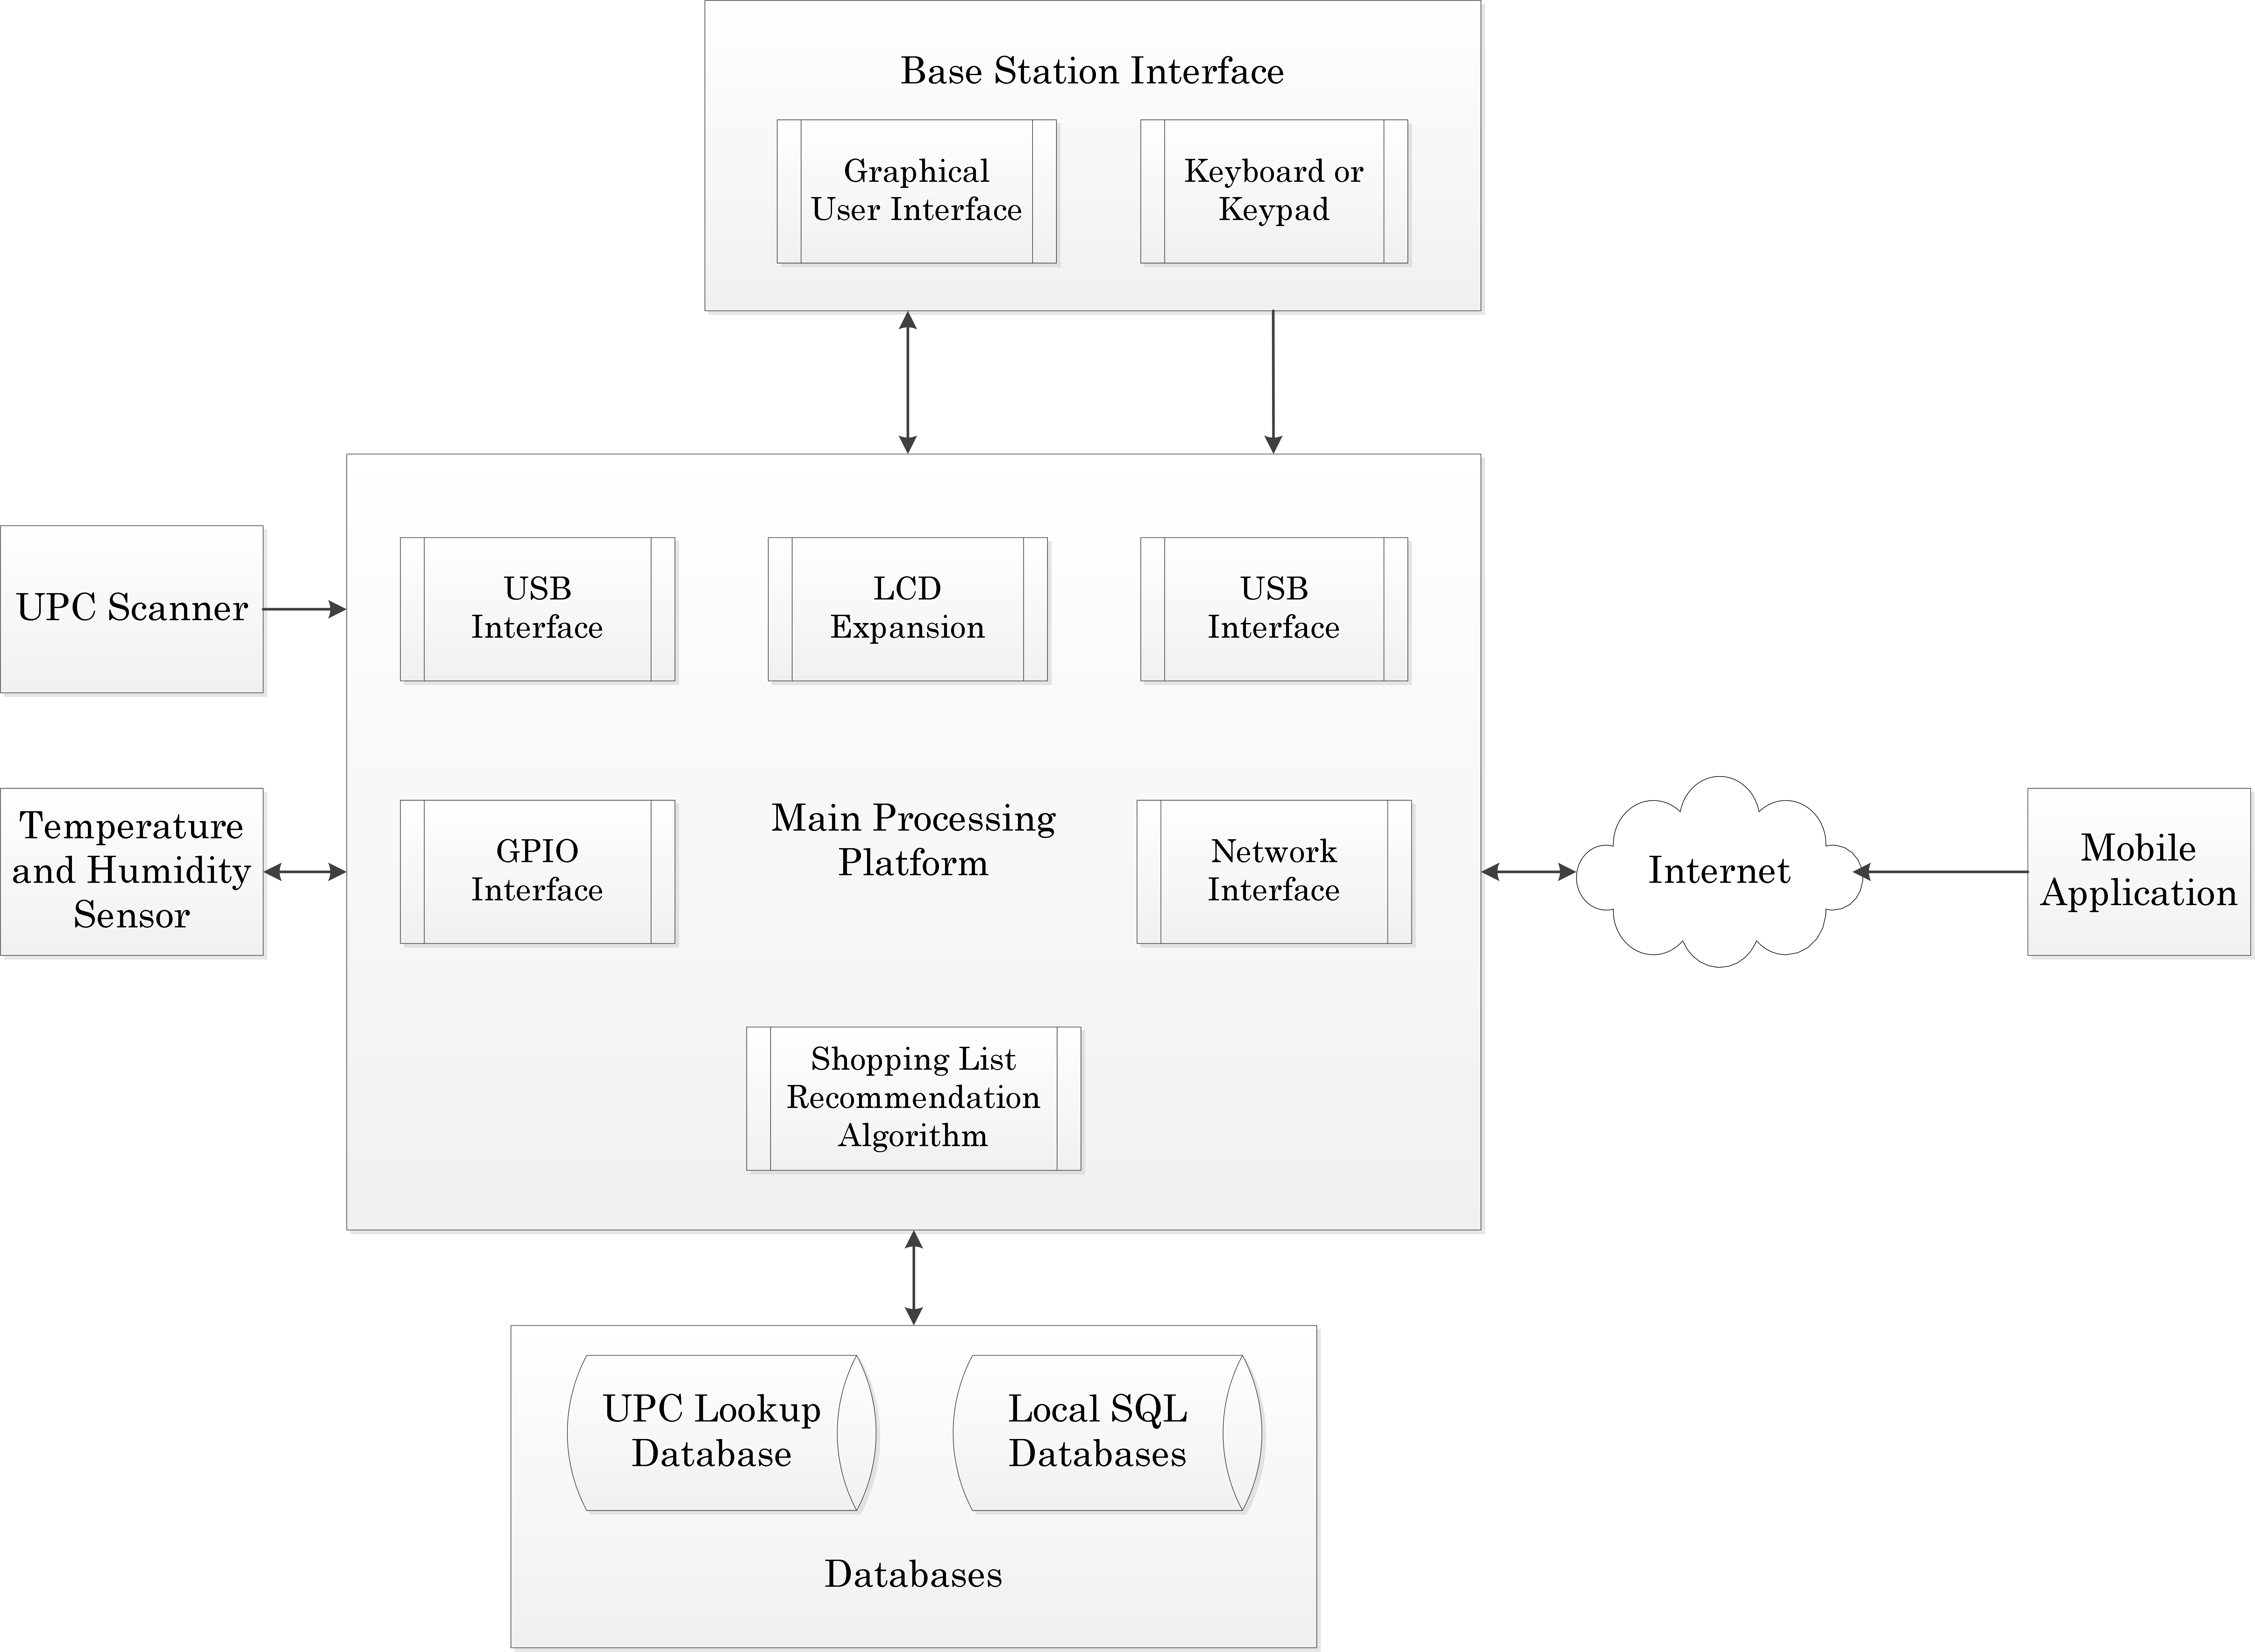
\includegraphics[scale=0.4]{../Graphics/FullSystemDiagram}
\caption{Full System Diagram}
\label{fig:fullsys}
\end{center}
\end{figure}
\newline \quad \newline
The majority of software developed will run on the Beagleboard, which will be the main processing platform for the Smart Refrigerator system. The Beagleboard will run the Angstrom operating system, a lightweight embedded Linux. A full Linux environment will be very conducive for software development and will greatly simplify connection with peripherals; the keypad or keyboard, as well as the UPC scanner, will be able to simply ``plug-and-play." The temperature sensor will require more effort, particularly to ensure the input and output voltage levels meet the specifications of the sensor and do not damage the Beagleboard. The Digilent Pmod TMP2 temperature sensor that will be used requires a 3.3V or 5V power supply and will output voltages as high as the supply voltage. The Beagleboard's I$^2$C interface supplies and receives voltages up to 1.8V only. To resolve this discrepancy, a BOB08745 Logic Level Converter will also be incorporated to interface between the Beagleboard and the temperature sensor.
\newline \indent \newline
A more detailed diagram of the Beagleboard subsystem is shown in Figure \ref{fig:basecode}. The figure shows all external connections to the Beagleboard as well as an internal separation of sub-components. The base station code will be inspired by the Model, View, Controller paradigm. A distinct module of code will create the user interface displayed on the Beagleboard's touchpad and will relay user interface events to a separate controller module. The controller sub-component will coordinate the various input events generated by the system. Input from the UPC scanner and keyboard will pass through this module and will then be transferred to the view. The controller is a necessary middleman in this process, since scanned UPC codes and user inputs must be shared with the model as well. The controller will also be responsible for handling input from the temperature and humidity sensor; this interaction will occur through a dedicated I$^2$C driver. The controller must also interact with the database structures and handle events from the network interface. The model itself will be distributed among the remaining modules; the content needed by the model will be stored within the databases, and the principal modeling task will occur within the expiration date and shopping list prediction sub-module.
\begin{figure}[h!]
\vspace{0.5cm}
\begin{center}
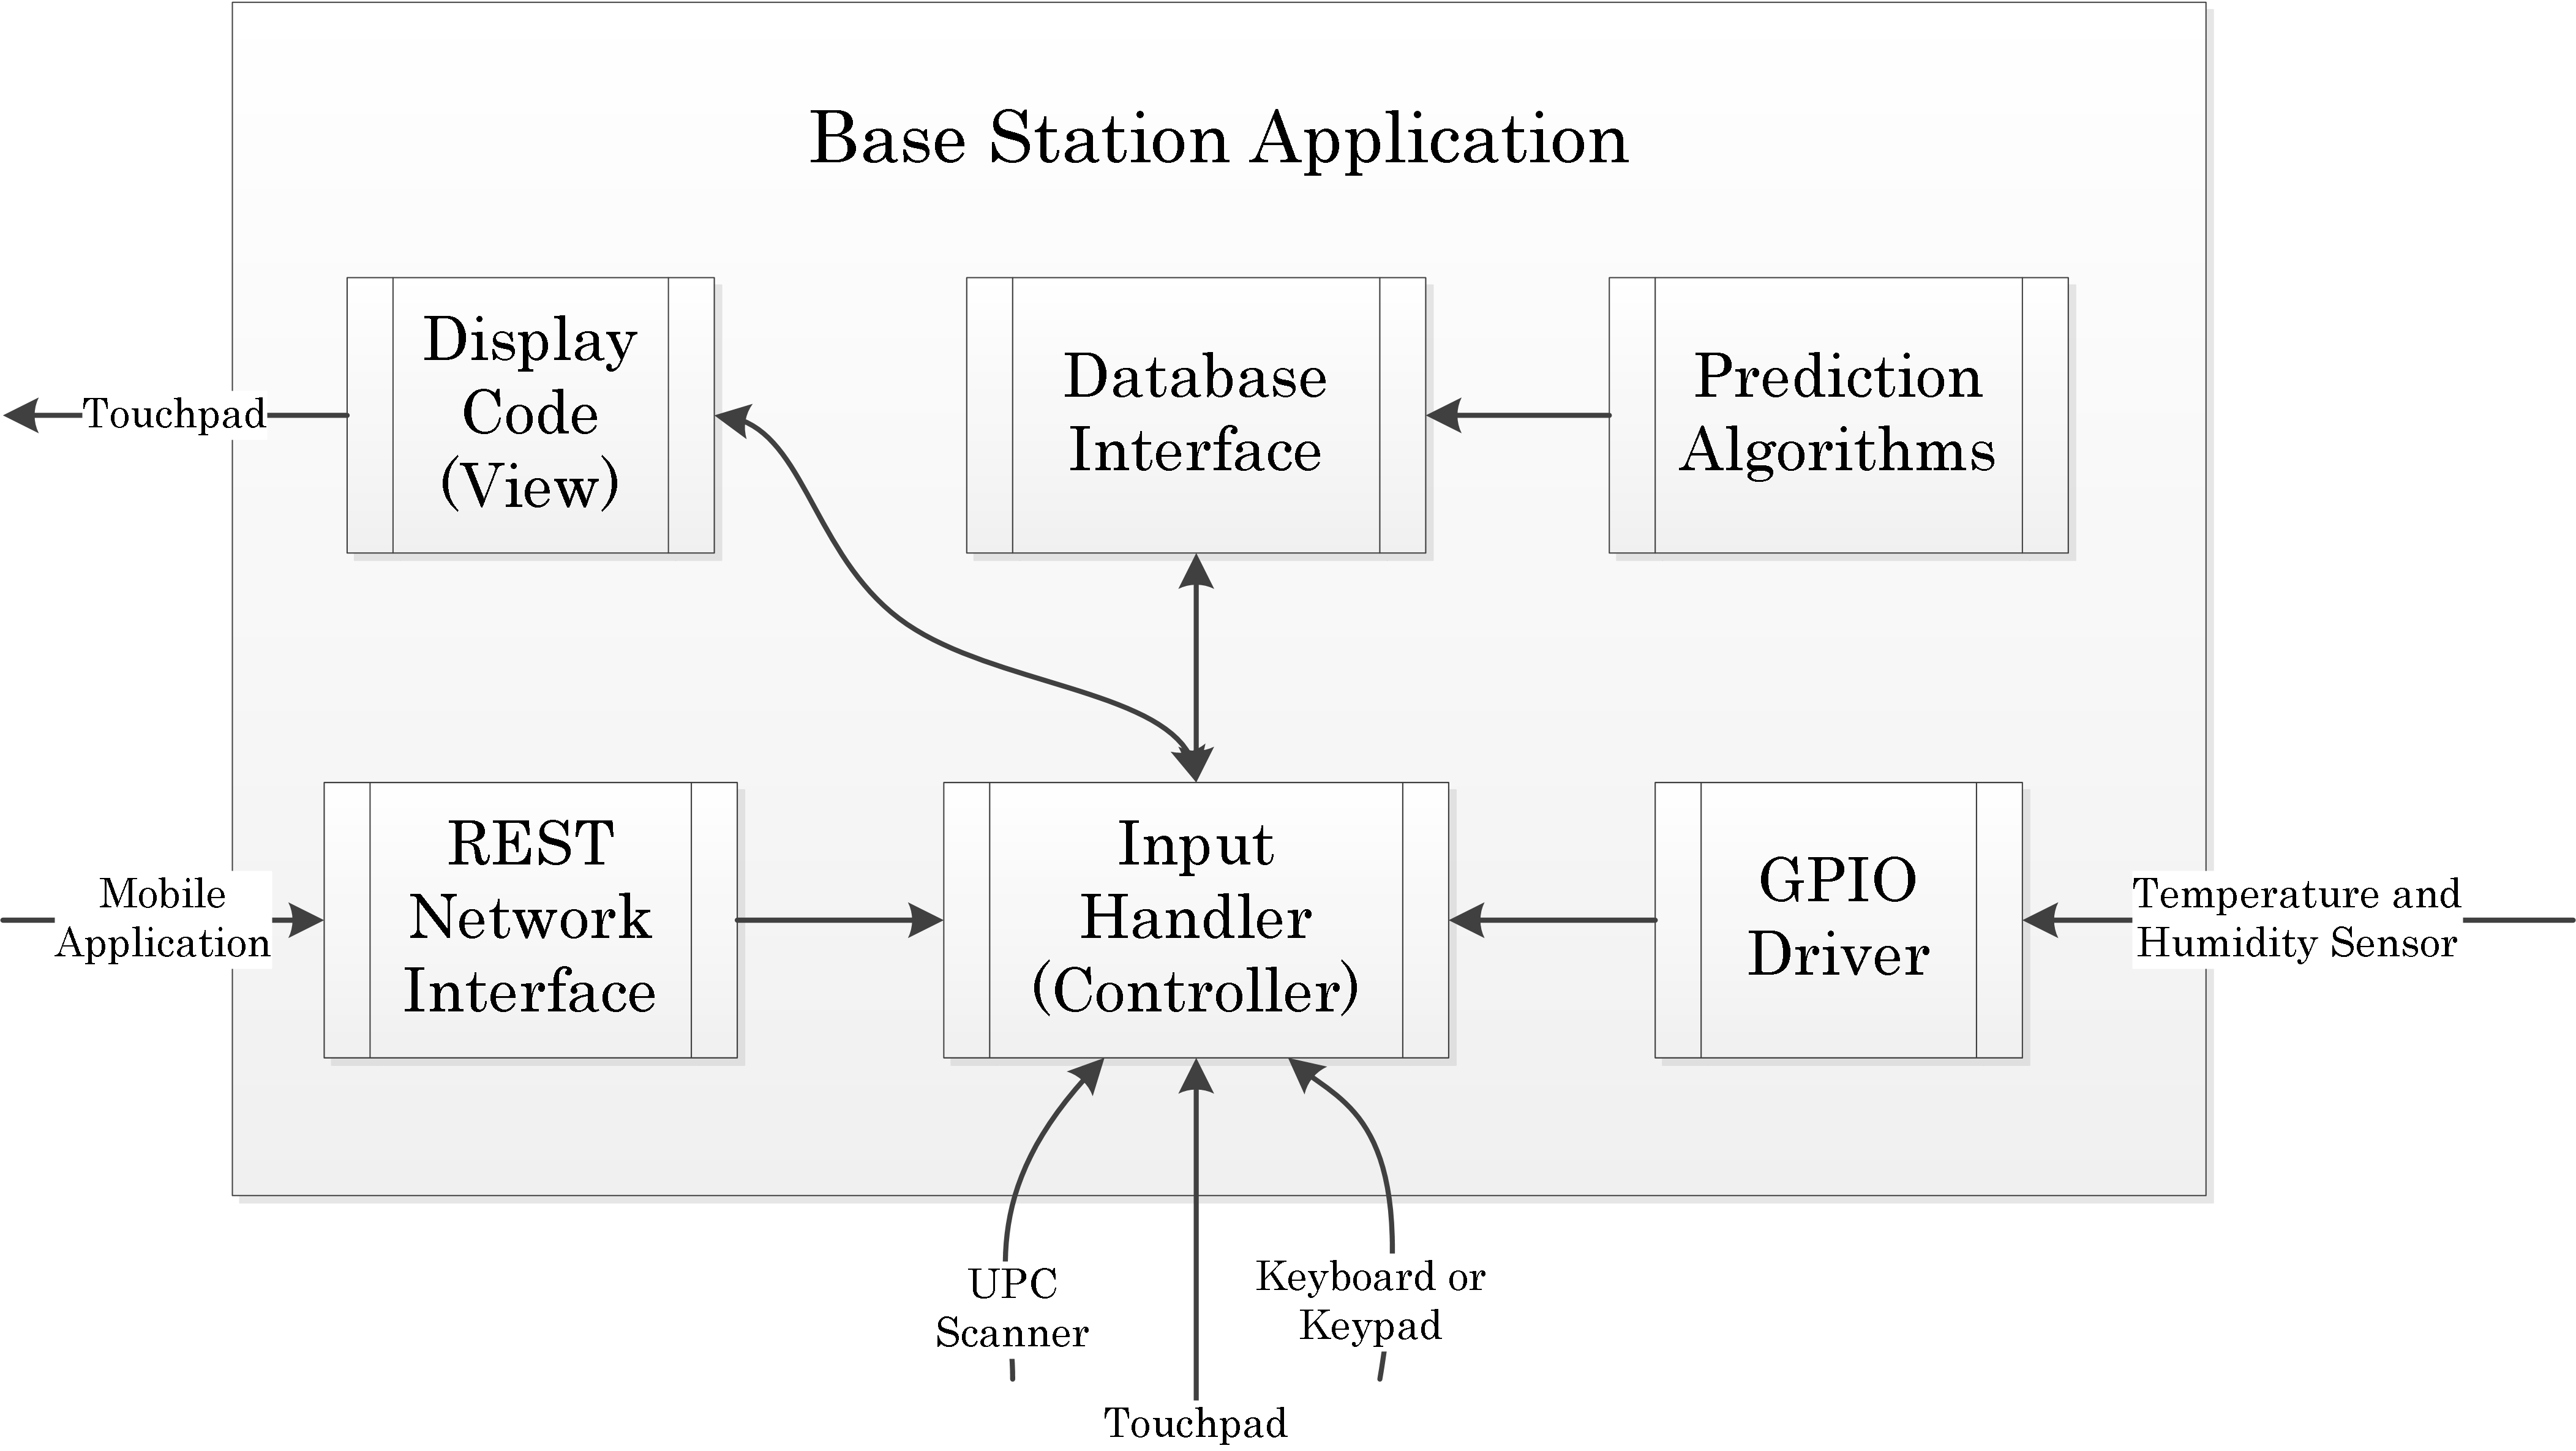
\includegraphics[scale=0.6]{../Graphics/BaseStation}
\caption{Beagleboard Subsystems}
\label{fig:basecode}
\end{center}
\end{figure}
\newline \quad \newline
\subsection{Base Station Code Package}
The base station application will be developed in Python using the TkInter user interface framework. Java was also given consideration as the primary language, since this could potentially increase consistency with the mobile application. However, Python is notoriously quick to develop with and was able to prototype the user interface rapidly. Effort will still be made to maintain consistency between the two user interfaces. To facilitate ease of use and a fluid user experience between the two applications, the interface layout should be preserved, and aesthetic differences should be minimized. Screen captures of the base station graphical user interface are shown in Figures \ref{mock1}, \ref{mock2}, \ref{mock3}. When designing the interface layouts, the constraints of a touch screen interface were considered; all buttons and tabs are intentionally large and easy to click. The product entry tab, shown in Figure \ref{mock1}, is the default tab, and provides feedback to the user while scanning items. The check in and check out buttons function as radio buttons to indicate whether the next scanned item will be interpreted as a new purchase or an item being removed from the current inventory. Since this tab is also be the default, a list of items closest to expiring is shown at the bottom to remind the user. The shopping list tab provides a straight-forward view of past shopping lists, organized by descending creation dates. The suggested list button will produce a new recommended shopping list. The current inventory tab simply lists items currently checked into the refrigerator and provides a reset function to clear the current inventory.
\pagebreak
\begin{figure}[h!]
\vspace{0.5cm}
\begin{center}
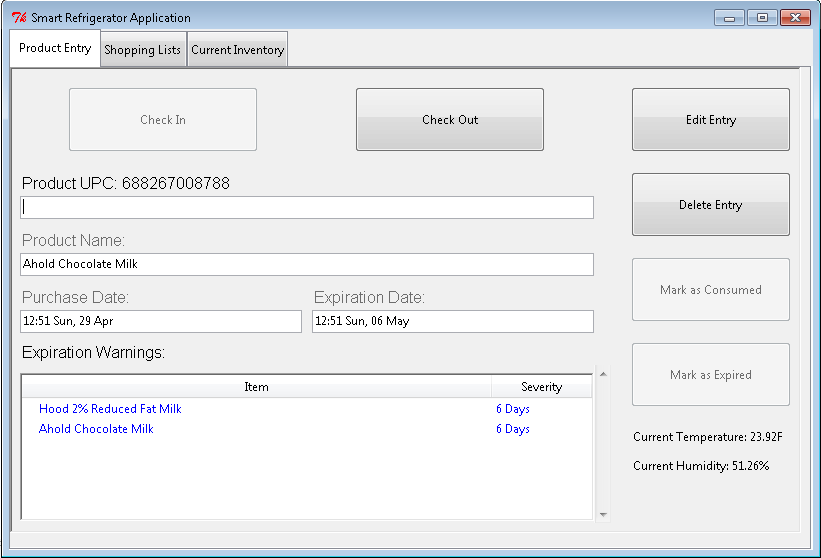
\includegraphics[scale=0.45]{../graphics/ProductEntry}
\caption{Product Entry Tab Layout}
\label{mock1}
\end{center}
\end{figure}

\begin{figure}[h!]
\begin{center}
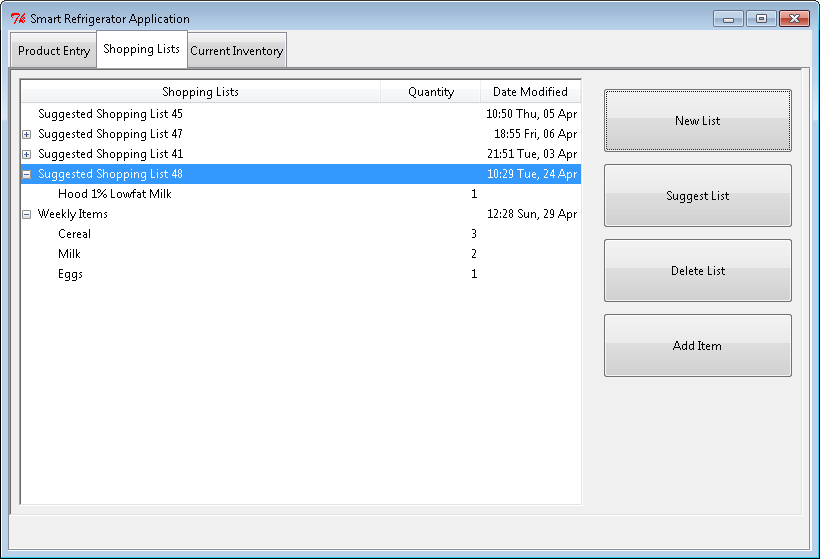
\includegraphics[scale=0.45]{../graphics/ShoppingLists}
\caption{Shopping List Tab Layout}
\label{mock2}
\end{center}
\end{figure}
\pagebreak
\begin{figure}[h!]
\vspace{0.5cm}
\begin{center}
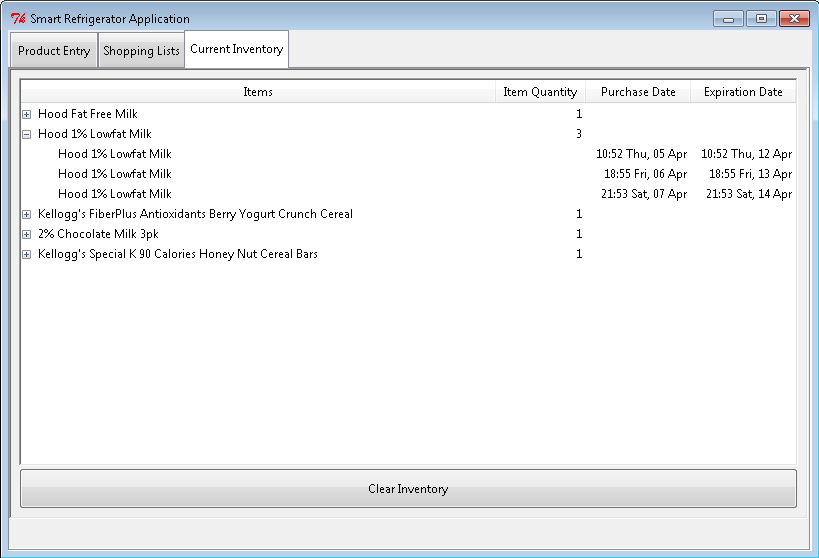
\includegraphics[scale=0.45]{../graphics/CurrentInventory}
\caption{Current Inventory Tab Layout}
\label{mock3}
\end{center}
\end{figure}

\quad \newline
\subsection{Mobile User Interface}
The mobile interface is divided into two similar tabs, one to view the current inventory and another to view shopping lists. Screen captures for the two mobile interface tabs are shown in Figures \ref{mob1}, and \ref{mob2}. Clicking an item in the inventory tab will display a list of all purchase dates for that item, as shown in Figure \ref{mob3}. Similarly, on the shopping list tab clicking an item will display a list of all items on that shopping list, as shown in Figure \ref{mob4}. The mobile application will be updated on a ``need to know" basis only. If additional items have been added to the inventory or new shopping lists have been created, the mobile application will not be notified until the user has opened the application and navigated to the appropriate tab. It is anticipated that the largest data exchanges will need to occur for the shopping lists, since they will require information from multiple items and additional top-level information about the lists. The mobile application will further improve data efficiency by not loading shopping list items until a list has been selected. Navigation to the shopping list tab will generate a query for the top-level information about new or updated shopping lists, but will not delve into the lists themselves to retrieve item information. Only once a list has been selected will complete updated information about its items be retrieved. This implementation will create additional latency while using the application; faster strategies include a single large update of all data upon launching the application or a background fetch of information while running the application. However, given the high costs of mobile data plans and the lack of widespread WiFi at most grocery stores, limiting the amount of data passed across the network interface is an important consideration for usability.
\newline \quad \newline
The mobile application should also be tolerant of interrupted connections, since telecommunication networks often have spotty coverage. To mitigate the impact of dropped connections, updates should be transferred from the Beagleboard to the mobile application in a sequence of short communications; a large number of small messages will be more robust than a small number of large messages. This structure will facilitate the ``need to know" distribution of information as well.
\newline \quad \newline
To actually communicate with the web interface a combination of HTTP requests, PHP, and JSON was used. The mobile application indicated what type of query to make to the web interface using an HTTP request. A snippet of PHP code on the server side would actually perform the query into the Beagleboard's MySQL databases and the results were formatted as a JSON string. The Android application parsed the JSON string and formatted the results into objects.

\subsection{Web Interface}
The actually web interface itself was hosted by a Cherokee web server running on the beagleboard. A simple HTML front end was also hosted in addition to the interface code for the mobile application. This interface consisted of two tables, one to show the current inventory and another listing the available shopping lists. The elements in the shopping lists table are links and clicking any shopping list will lead to another page showing a table with the items in that shopping list. Screen captures are shown for the web interface front end in Figures \ref{web1} and \ref{web2}.

\subsection{Database Definitions}
The various databases are implemented as MySQL databases on the Beagleboard. MySQL databases will certainly be reliable, and testing only ensured correct interaction with the databases. Figure \ref{fig:databases} illustrates the partitioning of data into the multiple tables stored on the Beagleboard. The most intuitive database is the Item Inventory Table, which stores the current contents of the refrigerator and their corresponding purchase and expiration dates. However, only the last purchase date is not be sufficient for the shopping list prediction algorithm, so a separate item history table stores all purchase dates indexed by UPC. The purchase dates are not stored as a list but just as separate rows in the table; the number of rows returned by a query indicates the number of purchase dates. A shopping list is included to store the top-level information about a shopping list: the ID,name, and creation date. The shopping lists also include a flag to indicate whether each shopping list was manually created or generated by the shopping list creation algorithm; the user may find this information useful when evaluating shopping habits. To coordinate between the table of items and the shopping lists themselves, an intermediate linking table was included to store the actual items included on a shopping list. This table is indexed by the shopping list identification number, and each row represents an item belonging to a shopping list. The number of rows returned by a query against a specific list ID indicates the number of items on that shopping list.
\begin{figure}[h!]
\vspace{0.5cm}
\begin{center}
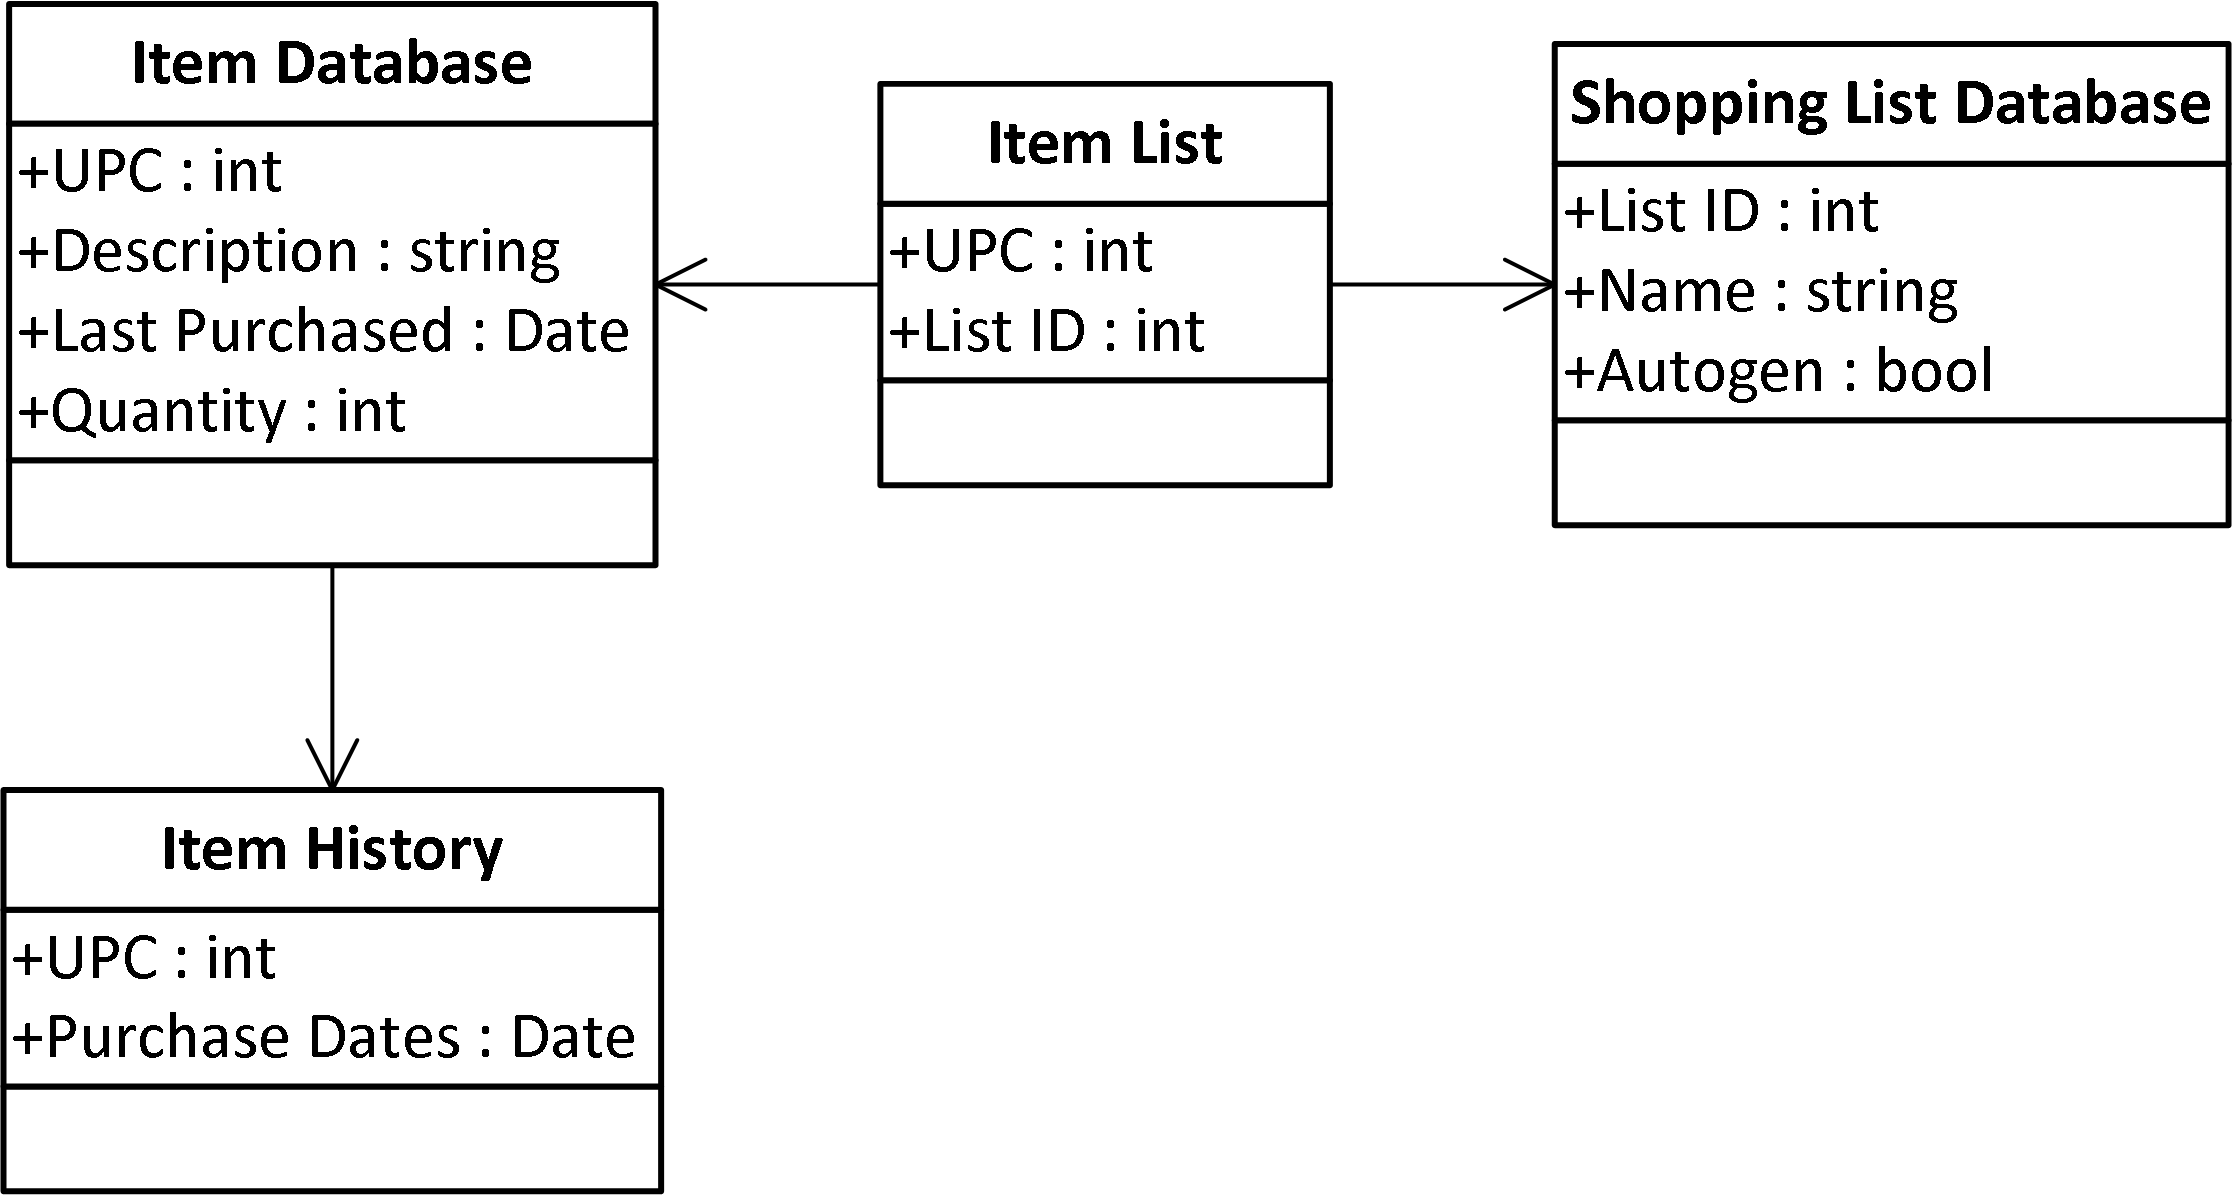
\includegraphics[scale=0.7]{../Graphics/Databases}
\caption{Separation of Information in Databases}
\label{fig:databases}
\end{center}
\end{figure}
\begin{description}
\item[Extensibility] -- The Smart Refrigerator system developed is only a first step toward tackling food waste; integration of the concepts in this prototype into a larger context could provide enormous utility. Possibly the expiration date and purchasing prediction systems could be improved and applied in commercial domains. Both small restaurants and national chains could benefit from more accurate shelf life predictions. The shopping list suggestion algorithm may also be improved by aggregating data from multiple users.
\item[Manufacturability] -- The Smart Refrigerator is a mainly software system and will therefore be easy to reproduce; the same code package could easily be mass-produced. However, the Beagleboard is a very general processing platform. If this prototype system were manufactured commercially, a more tailored and application specific platform could be desirable. The system does not have a true need for a  complete Linux environment, even though it is ideal for rapid development of a prototype.
\item[Reliability] - The components developed and tested externally, such as the Angstrom operating system, were assumed to be very robust in comparison with the modules developed specifically for this prototype. The user interfaces and prediction algorithms were both tested extensively, however in both cases it is difficult to eliminate the possibility of error. It was difficult to simulate all interrupted connection scenarios in testing and mobile interface likely did not encounter all possibilities and defects may have gone unnoticed. The shopping list recommendation algorithm was not exposed to all shopping habits in testing, and therefore may perform poorly in some untested scenarios. Fortunately, the system will not incur any damage from a failure and will not immediately endanger the user in event of a failure.
\item[Background] -- Experience with Linux based operating systems throughout the computer science sequence has been helpful. The computer science sequence and software engineering also have provided a valuable introduction to user interface development. The project does not contain significant hardware design, though skills learned in Interface and Digital Electronics may be useful in interfacing with the temperature and humidity sensor.
\item[Multidisciplinary Aspects] -- This prototype system requires coordination between hardware and software and requires a mixture of Computer Engineering and Software Engineering skills. However, multidisciplinary projects often carry a mechanical connotation and this system does not require integration of any mechanical components.
\end{description}
\section{Considerations}
The Smart Refrigerator system developed is a step toward promoting sustainability and good stewardship of natural resources. Both the New York Times articles mentioned in the statement of needs, and other reports \cite{times, aol}, indicate that approximately 27\% of all food available for consumption is lost to waste. A study published by the UN Food and Agriculture Organization declares the global percentage is even higher, totaling 1.3 billion tons or 33\% overall \cite{dutch}. The system designed will increase awareness about expiring items, with the goal of reducing these figures. Hugh Collins from AOL News speculates that food waste is dismissed subconsciously; many foods are cheap, and the average consumer does not think about the aggregated cost of these small wastes \cite{aol}. By providing reminders to the user, the Smart Refrigerator can remedy this source of waste by keeping the user aware of all their purchases. Expiration of food products themselves is not the only source of waste involved with grocery shopping. Making unnecessarily frequent trips to a store for forgotten or unexpected items also wastes resources. The shopping list recommendations provided by the Smart Refrigerator will hopefully mitigate waste here as well. A final consideration of the system is health and safety, by providing reminders about expiring products the risk of eating expired products will hopefully be decreased. 

\section{Cost Estimates}
We submitted a proposal to the ARM student design contest requesting a BeagleBoard-xM and power adapter. Our team received a BeagleBoard-xM at no cost, however the ULCD7 Lite display and power adapter were not provided and were purchased. We also already own many of the principle system components; the dorm room refrigerator, Android smart phone, and keyboard will not need to be purchased.
\begin{table}[h!]
\vspace{0.5cm}
\begin{center}
\caption{Cost Table}
\label{tab:cost}
\begin{tabular}{| p{3.0in} | p{1.5in} |p{1.5in} |}
\hline
Part & Retail Cost & Our Cost \\
\hline
BeagleBoard-xM & \$149 & \$0 \\
\hline
BeagleBoard-xM Power Adapter & \$26.33 & \$26.33 \\
\hline
Dorm Room Refrigerator & \$100 & \$0 \\
\hline
Android Smart Phone & \$100 & \$0  \\
\hline
ULCD7 Lite Display & \$151.50  & \$151.50 \\
\hline
UPC Barcode Scanner & \$40.67 & \$40.67 \\
\hline
USB Keyboard/Keypad & \$10 & \$0 \\
\hline
Digilent Pmod TMP2 Temperature Sensor & \$42.55 & \$0 \\
\hline
\hline
\textbf{Total Cost} & \$620.05 & \$271.05 \\
\hline
\end{tabular}
\end{center}
\end{table}

\section{Testing Strategy}
Testing of the Smart Refrigerator was divided into unit testing of the various subsystems and then top-level integration testing once the sub-systems had been connected. Some components used within the system, such as the Angstrom operating system and SQL database implementation, which have undergone extensive testing prior to use in our system, will be tested only to ensure proper configuration. The principle subsystems tested were the base station user interface, mobile user interface and network interface, expiration date and shopping list prediction algorithms, and integration with the BeagleBoard.

\subsection{Base Station User Interface Testing}
The main testing focus was placed on the user application, both the software running on the base station as well as the web and Android interfaces.  Unit testing was performed during development of each component, as well as integration testing of the final application. This subsection will focus on top-level testing of the base station user interface as a module, with tests particularly directed at the engineering specifications and user requirements. Tests directly motivated by the requirements specification and engineering specifications are listed below, and the test procedure completed is tabulated in Table \ref{tab:gui}.
\begin{itemize}
\item The user interface is required to be easy to use and intuitive; in order to verify this someone not involved in the project was enlisted to contribute to top-level testing of this sub-system. This also was also tested quantitatively; tests were performed to ensure the most used items are presented on the default tab, and the most frequently used controls are the most accessible.
\item The user interface provides access to the current inventory, which will be stored using an SQL database. The principal test effort at this step will be verifying integration of the display with the database, not verifying the storage of items themselves.
\item The user interface will provide both read and write access to shopping lists, also stored using an SQL database. Testing of this feature will again focus on the ability of the interface to query and modify database entries, not on the database implementation itself.
\item The user interface must provide a method to update expiration estimates. Testing of this subsystem will not verify that the update is reasonable or correct but simply verify that this user interface action triggers an update from the expiration prediction subsystem.
\item To achieve the principal goal of the system, the user interface must provide a notification of items about to expire. Testing of this subsystem will not verify that the expiration estimate is reasonable or correct, but simply that if triggered by the expiration prediction subsystem the user interface will display an indication.
\end{itemize}

\begin{table}[h!]
\vspace{0.5cm}
\caption{Base Station User Interface Test Cases}
\label{tab:gui}
\begin{tabular}{|c|p{3cm}|p{6cm}|c|c|c|c|c|}
\hline
\multicolumn{8}{|l|}{Test Writer: Steven Strapp} \\
\hline
\hline
\multicolumn{2}{|c|}{Test Case Name:} & \multicolumn{4}{|l|}{Base Station Interface Top-Level Unit Tests}& Test ID \#: & Base-01 \\
\hline
\multicolumn{2}{|c|}{Description:}& \multicolumn{4}{|p{8cm}|}{Verify that the base station user interface meets the requirement and engineering specifications. Some, such as usability will be evaluated qualitatively and are difficult to outline in this way.}&Type:&White Box\\
\hline
\hline
\multicolumn{8}{|l|}{Tester Information}\\
\hline
\multicolumn{2}{|c|}{Name of Tester:}&\multicolumn{4}{|l|}{Steven Strapp}& Date:& 04/29/12 \\
\hline
\multicolumn{2}{|c|}{Hardware Ver:}&\multicolumn{4}{|l|}{1.0}&Time: & 10:50\\
\hline
\hline
\multicolumn{2}{|c|}{Setup:}&\multicolumn{6}{|p{10cm}|}{User interface subsystem should be entirely integrated with prediction subsystems and SQL databases. System should begin without shopping lists or inventory. System date should be made mutable to facilitate quick simulation of expiration.} \\
\hline
\rotatebox{90}{Test \hspace{.2cm}}& Action& \multicolumn{1}{|p{6cm}|}{Expected Result} & \rotatebox{90}{Pass}& \rotatebox{90}{Fail} & \rotatebox{90}{N/A} & \multicolumn{2}{|p{3cm}|}{Comments}\\
\hline
1 & Enter test \newline product code & Switch to inventory tab,  entered product should be shown. Inventory should be otherwise empty. & X & & &\multicolumn{2}{|c|}{}\\
\hline
2 & Wait for test \newline product to nearly expire & Interface should display a notification indicating expiring item. & X & & &\multicolumn{2}{|p{4cm}|}{Item added to list of items near expiration on main tab.}\\
\hline
3 & Use interface to indicate product has not yet \newline expired & Verify that prediction sub-system is triggered to update its expiration estimate for this product. & X & & &\multicolumn{2}{|c|}{}\\
\hline
4 & Create fake \newline shopping list & Verify that list becomes accessible through base station and Android interface & X & & &\multicolumn{2}{|c|}{}\\
\hline
5 & Modify items on \newline fake shopping list & Verify that changes are retained and visible through base station or Android interface & X & & &\multicolumn{2}{|c|}{}\\
\hline
\end{tabular}
\end{table}
\pagebreak
\subsection{Mobile User Interface and Network Interface Testing}
The web and mobile interfaces will have their own set of tests, focused on basic functionality and interoperability on various platforms.  The web interface will be tested on the most popular browsers (Google Chrome, Firefox, and Internet Explorer), as well as some of the most popular mobile platforms (Android, WebOS, and iOS).  The Android interface will need to be tested on various versions of the operating system.  At a minimum, major versions between 2.1 and 4.0 will be tested.  

\begin{table}[h!]
\caption{Mobile App Tests}
\label{tab:mobApp}
\begin{tabular}{|c|p{3cm}|p{6cm}|c|c|c|c|c|}
\hline
\multicolumn{8}{|l|}{Test Writer: Ben Reeves} \\
\hline
\hline
\multicolumn{2}{|c|}{Test Case Name:} & \multicolumn{4}{|p{8cm}|}{Downloading large database updates 
over an \newline intermittent network connection}& Test ID \#: & Mob-01 \\
\hline
\multicolumn{2}{|c|}{Description:}& \multicolumn{4}{|p{8cm}|}{Ensure that the database is correctly downloaded
even if the device's network connection is interrupted. This could be due to 
loss of service, a disabled network adapter, or the device powering down.}&Type:&White Box\\
\hline
\hline
\multicolumn{8}{|l|}{Tester Information}\\
\hline
\multicolumn{2}{|c|}{Name of Tester:}&\multicolumn{4}{|l|}{Ben Reeves}&Date: & 4/19/12\\
\hline
\multicolumn{2}{|c|}{Hardware Ver:}&\multicolumn{4}{|c|}{1.0}&Time: 10:30& \\
\hline
\hline
\multicolumn{2}{|c|}{Setup:}&\multicolumn{6}{|p{12cm}|}{System should have a fresh 
install of the application and no previous copies of the database downloaded.} \\
\hline
\rotatebox{90}{Step \hspace{.2cm}}& Action& \multicolumn{1}{|p{6cm}|}{Expected 
Result} & \rotatebox{90}{Pass}& \rotatebox{90}{Fail} & \rotatebox{90}{N/A} & 
\multicolumn{2}{|p{3cm}|}{Comments}\\
\hline
1 & Initiate download \newline update of the \newline database & System should connect to the server 
  and begin downloading. & X & & &\multicolumn{2}{|c|}{}\\
\hline
2 & Sever device's \newline network \newline connection & System should pause the download upon sensing 
  the interrupted connection. & X & & &\multicolumn{2}{|c|}{}\\
\hline
3 & Reconnect device \newline to the network & System should resume download of the database 
  & & & X &\multicolumn{2}{|p{3cm}|}{Download is \newline restarted, not \newline resumed.}\\
\hline
4 & Allow update to \newline complete & System should download the remaining portion of the 
  database& X & & &\multicolumn{2}{|c|}{}\\ 
\hline
\end{tabular}
\end{table}
\pagebreak

\begin{table}[h!]
\vspace{0.5cm}
\caption{UI Usability Test}
\label{tab:usability}
\begin{tabular}{|c|p{3cm}|p{6cm}|c|c|c|c|c|}
\hline
\multicolumn{8}{|l|}{Test Writer: Ben Reeves} \\
\hline
\hline
\multicolumn{2}{|c|}{Test Case Name:} & \multicolumn{4}{|l|}{UI Usability Test}& Test ID \#: & UI-01 \\
\hline
\multicolumn{2}{|c|}{Description:}& \multicolumn{4}{|p{8cm}|}{Ensure that the both the web and mobile 
 versions of the User Interface are accessible and intuitive.}&Type:&White Box\\
\hline
\hline
\multicolumn{8}{|l|}{Tester Information}\\
\hline
\multicolumn{2}{|c|}{Name of Tester:}&\multicolumn{4}{|l|}{Ben Reeves}&Date: 4/19/12& \\
\hline
\multicolumn{2}{|c|}{Hardware Ver:}&\multicolumn{4}{|c|}{1.0}&Time:& 11:45 \\
\hline
\hline
\multicolumn{2}{|c|}{Setup:}&\multicolumn{6}{|p{12cm}|}{System should be representative of one which is in
active use; that is, its database should contain both shopping lists and grocery items associated with them.} \\
\hline
\rotatebox{90}{Step \hspace{.2cm}}& Action& \multicolumn{1}{|p{6cm}|}{Expected 
Result} & \rotatebox{90}{Pass}& \rotatebox{90}{Fail} & \rotatebox{90}{N/A} & 
\multicolumn{2}{|p{3cm}|}{Comments}\\
\hline
1 & System is given to a user unfamiliar with its operation and submitted to stress testing & 
  User should experience little difficulty navigating the application and experience no bugs, freezes, or crashes. 
  & X & & &\multicolumn{2}{|c|}{}\\
\hline
\end{tabular}
\end{table}
\pagebreak

\begin{table}[h!]
\vspace{0.5cm}
\caption{UI Interoperability Test}
\label{tab:interop}
\begin{tabular}{|c|p{3.5cm}|p{5.5cm}|c|c|c|c|c|}
\hline
\multicolumn{8}{|l|}{Test Writer: Ben Reeves} \\
\hline
\hline
\multicolumn{2}{|c|}{Test Case Name:} & \multicolumn{4}{|l|}{UI Interoperability Test}& Test ID \#: & UI-02 \\
\hline
\multicolumn{2}{|c|}{Description:}& \multicolumn{4}{|p{7.5cm}|}{Ensure that the both the web and mobile \newline
 versions of the User Interface are fully \newline compatible with popular browsers.}&Type:&\multicolumn{1}{|p{1cm}|}{White \newline Box}\\
\hline
\hline
\multicolumn{8}{|l|}{Tester Information}\\
\hline
\multicolumn{2}{|c|}{Name of Tester:}&\multicolumn{4}{|c|}{Ben Reeves \& Steven Strapp}&Date: & 4/20/12\\
\hline
\multicolumn{2}{|c|}{Hardware Ver:}&\multicolumn{4}{|c|}{}&Time: & 10:40\\
\hline
\hline
\multicolumn{2}{|c|}{Setup:}&\multicolumn{6}{|p{11cm}|}{System should be representative of one which is in
active use; that is, its database should contain both shopping lists and grocery items associated with them.} \\
\hline
\rotatebox{90}{Step \hspace{.2cm}}& Action& \multicolumn{1}{|p{6cm}|}{Expected 
Result} & \rotatebox{90}{Pass}& \rotatebox{90}{Fail} & \rotatebox{90}{N/A} & 
\multicolumn{2}{|p{1cm}|}{Comments}\\
\hline
1 & Interface is accessed via Mozilla Firefox and subjected to stress testing 
  & Interface is displayed properly, no artifacts or misplaced \newline elements apparent.
  & X & & &\multicolumn{2}{|c|}{}\\
\hline
2 & Interface is accessed via Google Chrome and subjected to stress testing 
  & Interface is displayed properly, no artifacts or misplaced \newline elements apparent.
  & X & & &\multicolumn{2}{|c|}{}\\
\hline
3 & Interface is accessed via Microsoft \newline Internet Explorer \newline and subjected to \newline stress testing 
  & Interface is displayed properly, no artifacts or misplaced \newline elements apparent.
  & X & & &\multicolumn{2}{|c|}{}\\
\hline
4 & Interface is accessed via Android 2.3 and subjected to stress \newline testing 
  & Interface is displayed properly, no artifacts or misplaced \newline elements apparent. 
  & X & & &\multicolumn{2}{|c|}{}\\
\hline
5 & Interface is accessed via Android 4.0 and subjected to stress \newline testing 
  & Interface is displayed properly, no artifacts or misplaced \newline elements apparent.
  & X & & &\multicolumn{2}{|p{3cm}|}{Web interface has small break \newline in table with \newline default browser, \newline not critical.}\\
\hline
\end{tabular}
\end{table}
\clearpage

\subsection{Shopping List and Expiration Prediction Test}
Testing of the expiration prediction and shopping list prediction subsystems will be difficult if the system's date can not be adjusted artificially; testing should occur over a few minutes rather than a series of days. For expiration date testing, the system's date should be easy to change artificially, so products appear to expire very quickly. The intelligence of the system can then be tested by providing feedback that test products expired more or less quickly than expected, and evaluating the updated predictions. By simply accelerating the rate with which the system changes date, this subsystem can be tested without adding specific test products with low shelf lives and without changing the algorithms to update more frequently. A set of tests is listed for this subsystem below.
\begin{itemize}
\item Enter a product code and verify that the expiration date system is initialized with recommended ``rule of thumb" value.
\item Provide feedback indicating that a product expired before estimate and validate that the estimate is decreased. Also validate the opposite case: providing feedback that a product had not yet expired on estimated date should increase the estimate.
\item Enter a product code and advance the system time until the product is nearly expired. Verify that the prediction subsystem has indicated to controller that the product is nearing expiration.
\item Rescan a product code after regular intervals, indicative of uni-modal shopping habits. Verify that the system recommends the product should be purchased again on this mode. Date may be artificially advanced to facilitate quick testing.
\item Continue from the previous case and add outlier shopping habits. Validate that system continues to recommend purchasing the product again on the mode.
\item Enter various products with different purchasing habits. Verify that the system recommends purchasing the products with the highest probabilities.
\item Rescan a product code after regular intervals, then add significant variation. Observe that system attempts to track  the variation in habits.
\item Rescan a product code after varying intervals, indicative of bi-modal shopping habits. Verify that the system recommends purchasing the product on both modes.
\end{itemize}
\subsection{Integration with BeagleBoard}
Preliminary testing will focus on the BeagleBoard itself and its ability to interact with the desired peripherals.  The system will require an LCD screen, a USB barcode scanner, a network connection, a keypad, and temperature/humidity sensor.  Basic functionality of these components will be tested thoroughly during development, as well as during final system testing. 
\newline \quad \newline
The SQL database used to store all data for the system will be tested once the core of the user application has been coded.  Test scripts will be written to populate the databases with fake data in order to ensure that the database is configured as desired, and to verify that the user application is properly communicating with the database alongside the web interface.
\newline \quad \newline
It is difficult to outline exactly what testing will be required for the processing platform, since it is unclear what compatibility issues will arise that would not be presented by a conventional platform, where ideally the system would be entirely ``plug and play." However, listed below is a baseline sequence of tests.
\begin{itemize}
\item Verify that the BeagleBoard, with power adapter, can power all peripheral devices reliably so that no sporadic failures occur; this will be performed as an endurance test.
\item Verify that MAC address of Ethernet interface can be statically assigned and the BeagleBoard can be pinged reliably; this will be performed as an endurance test, cycling power or disconnecting the board multiple times.
\item Verify that the BeagleBoard can reliably interface with the USB scanner and USB keypad; these tests should be performed by writing to a text editor or another program external to the user interface to isolate failures.
\item Verify that the BeagleBoard consistently receives accurate temperature and humidity measurements from the sensor, via the general purpose input/output pins. The measurements should be verified with an external sensor.
\item Verify that the touchscreen display accurately records users clicks and controls the pointer; tested outside of the user interface to isolate failures.
\item Verify that touchscreen accurately displays the graphical user interface without artifacts or distortion consistently, and ensure all controls on the display are accessible.
\end{itemize}

\section{Risks}
The risks unresolved in the prototype system are best grouped by subsystem. Some unresolved risks are simply due to unknown availability of parts, others require further exploration, and still others are more fundamental risks.
\begin{description}
\item[Availability of LCD Display] -- The ULCD7 Lite is the preferred choice for the display to accompany the Beagleboard. The 7-inch resistive touchscreen is designed to work with the Beagleboard and has drivers built into the Angstrom Linux distribution. However, the touchscreen does not seem to be stocked by online suppliers and our request through the Arm Developer Day proposal process is still pending. Since the Beagleboard provides a DVI-D and S-video output, this risk could be mitigated using a traditional computer monitor if the preferred touch screen is not available. The availability of these alternate interfaces also facilitates development while waiting for the desired part. However, since the base station display is a critical system component, if this risk is not resolved shortly one of the less desirable alternatives will have to be selected.
\item[Mobile Application Data Exchange] -- Exchanging inventory and shopping list data with the mobile application presents two risk areas: the amount of data plan usage required and interrupted network connections. These risks are partially mitigated by the design, which exchanges data in small increments on a ``need to know" basis only; however the degree to which these risks are truly problematic is not know. For development, the smart phone can be connected with WiFi instead of a costly data connection; however, the data requirements should be tested early in development to ensure this risk does not become a latent problem. Interrupted connections are considered in the design, but the effectiveness of the design will be difficult to measure since it may be difficult to repeatedly interrupt the data connection.
\item[Practicality of Prediction Algorithms] -- The shopping list prediction algorithm outlined appears optimal for the test data considered. However, the analysis performed did not consider a large sample of shoppers, and the conclusions drawn may not be appropriate for a larger population. Also, the prediction algorithm outlined will not perform well with only a few samples; it is unclear how unacceptable this warm-up period will appear to end users. The strategy presented is also quite heavy-handed and may be superfluous for this prototype system. The system will not serve as an effective shopping aid without an accurate prediction system, but a prototype may be acceptable with a much simpler system requiring significantly less effort.
\item[Efficiency of Database Access] -- Efficient practices for database access were not known or considered when partitioning information into separate tables. Efficiency was also not considered when developing the schema for the databases. For example, using the same database to store all possible items and the current inventory may be an inefficient choice. This strategy requires looking over all elements and extracting only those with non-zero quantities. If the system were extended to large commercial applications, or if the Beagleboard were replaced with a more cost-efficient and less powerful alternative, this organization may become a significant risk.
\end{description}

\begin{table}[h!]
\caption{Summary of Risks}
\label{tab:risksum}
\begin{center}
\begin{tabular}{|p{3cm}|p{12cm}|}
\hline
Risk & Comments \\
\hline
Availability of \newline LCD Display & The ULCD7 Lite display took several weeks to procure. However, this delay did not significantly effect the project time line and this risk was averted. \\
\hline
Mobile \newline A1pplication Data Exchange & There was an initial concern that the amount of data exchanged with the mobile application would be problematic. This risk did not impact testing for our simple prototype system but may remain a latent issue if the system were expanded to a larger scale. \\
\hline
Practicality of \newline Prediction Algorithms & There was initial concern that the shopping list prediction algorithms would take a significant amount of development time at the expense of areas that would be more obvious to an end-user. However, using SciPy this risk was absolved. \\
\hline
Efficiency of \newline Database Access & This Risk appeared more problematic with the original database schema, the schema was updated during design to resolve this risk. \\
\hline
\end{tabular}
\end{center}
\
\end{table}

\pagebreak
\section{Milestones}
\begin{table}[h!]
\begin{center}
\begin{tabular}{| p{3.5 cm} | p{2 cm} | p{2 cm}| p{2 cm} | p{5 cm} | }
\hline
\textbf{Milestone} & \textbf{Scheduled Date} & \textbf{Assigned} & \textbf{Modified Date} & \textbf{Comments} \\
\hline
BeagleBoard \newline procured & February 10, 2012 & SS & NA & Complete \\
\hline
Angstrom operating system running on board & February 24, 2012 & DS & NA & Complete \\
\hline
Peripherals properly interfacing with \newline board & March 02, \newline 2012 & DS & April 27, \newline 2012 & Complete. Touch screen Angstrom image works for both touch screen and temperature sensor. \\
\hline
Basic mobile UI, \newline suitable for \newline debugging & March 09, \newline 2012 & BR & NA & Complete \\
\hline
Basic base station UI, suitable for \newline debugging & March 09, \newline 2012 &SS & NA & Complete \\
\hline
Database I/O \newline configured & March 16, \newline 2012 & DS &  March 23, \newline 2012 & Complete. MySQL databases configured, can be accessed with Python application. \\
\hline
Testing and \newline integration of \newline temperature and \newline humidity sensor & March 16,  \newline 2012 &SS/DS & April 27, \newline 2012 & Unable to interact with one wire sensor using Beagleboard GPIO and level shifter. Replacement I$^2$C temperature sensor from Dr. Mondragon works correctly. \\
\hline
Database and web server hosted by\newline Beagleboard & March 16, \newline 2012 & DS & NA & Complete \\
\hline
Beagleboard \newline touchscreen display procured & March 16, \newline 2012 & DS & NA & Complete \\
\hline
Mobile application integrated with web server & March 30, \newline 2012 &BR & April 20, \newline 2012 & Complete\\
\hline
User profiling and statistical analysis & March 30,\newline 2012 & SS & April 6, \newline 2012 & Complete\\
\hline 

\end{tabular}
\end{center}
\end{table}

\begin{table}[h!]
\vspace{0.5cm}
\begin{center}
\begin{tabular}{| p{3.5 cm} | p{2 cm} | p{2 cm}| p{2 cm} | p{5 cm} | }
\hline
\textbf{Milestone} & \textbf{Scheduled Date} & \textbf{Assigned} & \textbf{Modified Date} & \textbf{Comments} \\
\hline
Shopping lists, item modification, basic \newline settings & March 30, \newline2012 & SS & & Complete. Added context \newline menus and hidden \newline ``administrator" panel. \\
\hline
Updated base \newline station UI & April 6,\newline 2012 & SS & & Complete, awaiting review by team or outside testers.\\
\hline
Updated mobile \newline application & April 6, \newline2012 & BR & April 20, \newline 2012& Complete\\
\hline
Integration testing \newline and system \newline verification & April 13, \newline2012 & BR & April 27, \newline2012& Complete\\
\hline
Web interface \newline development & April 20, \newline 2012 & SS & & Complete. Does not look \newline flashy but is effective and \newline functional. \\
\hline
System testing and demo preparation & April 20, \newline2012 & SS & April 27, \newline2012& Complete\\
\hline
Project Website & May 3, 2012 & SS & & Complete\\
\hline
Project Demo & May 3, 2012 & Team & & \\
\hline
Imagine RIT Demo & May 5, 2012 & Team & &\\
\hline
\end{tabular}
\label {MilestoneTable}
\end{center}
\end{table}

\pagebreak

\quad \newline \quad

\subsection{Gantt Chart}
\begin{figure}[h!]
\begin{center}
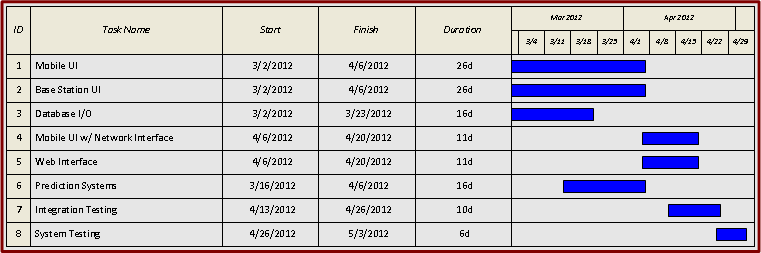
\includegraphics[scale=0.65]{../Graphics/GanttChart}
\caption{Project Gantt Chart}
\end{center}
\end{figure}

\section{Perspective}
The design of the final project adhered to the original proposal, however some of the implementations themselves changed. Some aspects of the system, such as the web user interface and database organization, were not thoroughly enough defined in the proposal and were not clear until the actual implementation. Difficulties and deviations from the original proposal are organized into subsections below.

\subsection{Base Station Code Package}
The most significant change in the base station code package was the programming language used; the original proposal declared C++ along with the Qt user interface framework, whereas Python and the Tk framework were eventually used. Python is much quicker to develop and the Tk allows for very quick creation of user interfaces. Python was also an advantageous choice for the prediction subsystems, the scientific computing library SciPy provides clustering and kernel density estimator code; both of which were considered as options for the shopping list recommendation system. The prediction system itself was revised after considering implementation with MySQL databases. The clustering strategy initially chosen during conception selection became undesirable in that it required clustering information to be stored in the database, and the number of cluster were not known a priori. Alternatively, the clustering could have been performed again at every prediction step however this was computation undesirable. Once database storage was considered in the concept selection a non-parametric estimate appeared optimal instead.
\newline \quad \newline
The user interface design followed the mock-ups very closely. The only significant change was to remove the expiration warning pop-ups and replace them with a list of high risk items on the main panel. Once the GUI was created and experimented with it became clear that by only showing a pop-up it was too easy to forget the warning after the pop-up had been cleared. A list of items near expiration on the main window prevents users from forgetting items that had been identified as nearing expiration.
\subsection{Web Interface}
The specifications for the web interface were not clearly defined in the original proposal, and expectation for this interface varied between team members. The expectation and implementation for this interface was not resolved until initial implementation. The web interface was implemented as a simple HTML page with embedded PHP snippets to query the databases hosted by the Beagleboard.

\subsection{Mobile Interface}
The initial plan outlined in the proposal was for the mobile application to interact with the Beagleboard through the same web interface. However, part way through development it was suggested that it might be simpler to interact directly with the remote databases on the Beagleboard. Attempts were made to connect to the databases with an object-relational mapping without any success, and it was later discovered that Android does not support remote database access. Instead, the design reverted back to the original plan. Another small PHP snippet on the Beagleboard's web server was included to respond to HTML post requests, access the database, and return result to the Android application. The Android application would issue a post request indicating which tabel should be accessed, the server side PHP would perform this query and return results as a JSON string. The Android application parsed the JSON string and converted the returned values into Java objects. Aside from this indecision, the Android develop proceeded as expected.

\subsection{Beagleboard Integration}
A number of integration issues arose while using the Beagleboard. The first issue encountered was with the Python base station code package. The shopping list prediction system used the SciPy library, however prebuilt binaries for this library are not available for ARM architectures. Compiling this package from source was unexpectedly difficult and required resolution of many dependencies. Next, the temperature sensor initially purchased, an RHT03, could not be interfaced with the Beagleboard. The RHT03 used a custom one wire interface that enforced very accurate timing requirements; the Beagleboard, running a non real-time operating system was not able to meet these requirements. Attempts were made to use more accurate timers or interrupts from the GPIO pins but neither of these methods accurately retrieved information from the sensor. Instead, an I$^2$C temperature sensor was obtained from Dr. Mondragon which worked trivially. Finally, the ULCD7 Lite touchscreen was initially only partially functional with the Angstrom image used; the display worked but would not respond to touch. Investigation revealed that additional modules needed to be compiled in with the Angstrom kernel. Instead of pursuing this option, the Angstrom image provided for the temperature sensor was used and the components developed on the earlier image was reinstalled on the touch screen image. This strategy required repeating installations and configurations but also appeared to be the option that was simplest and most likely to succeed.


\addcontentsline{toc}{section}{10\hspace{.090in} References}
\begin{thebibliography}{9}
\bibitem{times}
Martin, Andrew. ``One Country's Table Scraps, Another Country's Meal." New York Times. N.p., 18 May 2008. Web. 26 Jan 2012. 
\url{http://www.nytimes.com/2008/05/18/weekinreview/18martin.html?pagewanted=all}.
\bibitem{lg}
Ridden, Paul. ``LG launches first Smart-Grid appliance: the Smart Fridge." gizmag. N.p., 27 Apr 2011. Web. 29 Jan 2012. \url{<http://www.gizmag.com/lg-smart-fridge/18502/>}.
\bibitem{aol}
Collins, Hugh. ``Study: US Food Waste Is a Huge Energy Drain." AolNews. N.p., 02 Oct 2010. Web. 29 Jan 2012. \url{<http://www.aolnews.com/2010/10/02/study-american-food-waste-is-a-huge-energy-drain/>}.
\bibitem{dutch}
Ramaker, Rob. ``Food waste is hard to combat." Resource. N.p., 26 Jan 2012. Web. 29 Jan 2012. \url{<http://resource.wur.nl/en/wetenschap/detail/food_waste_is_hard_to_combat/>}.
 \end{thebibliography}

\end{document}
